\documentclass[a4paper, 11pt, twoside]{report}
\usepackage[a4paper]{geometry}
\usepackage{lmodern}
\usepackage{textcomp}
\usepackage{url}
\usepackage{float}
\usepackage{booktabs}
\usepackage{longtable}
\usepackage{makeidx}
\usepackage{fancyhdr}
\usepackage[times]{quotchap}
\usepackage{tikz}
\usepackage{multirow}
\usepackage{version}
\usepackage{tcolorbox}
\usepackage{listings}
\usepackage{xcolor}
\usepackage{hyperref}
\usepackage[T1]{fontenc}
\usepackage{graphicx} % Required for inserting images
\usepackage{hyperref}
\usepackage{amsmath, amsfonts}
\usepackage{apalike}
\usepackage{mathtools}
\usepackage{minted}
\usepackage{caption}
\usepackage{subcaption}
\usepackage{rotating}
%\usepackage[acronym]{glossaries-extra}

\newcommand{\dd}{\mathrm{d}}
\renewcommand{\L}{\mathcal{L}}
\renewcommand{\Vec}{\mathbf}
\newcommand{\mytitle}{Application of Physics-Informed Neural Networks for Galaxy Dynamics}
\newcommand{\myname}{Lucas Barbier-Goy}
\newcommand{\mysupervisor}{Prof. Dr. Marco Landoni \& Dr. Fabio Rigamonti}
\newcommand{\mydate}{May 25\textsuperscript{th}}

\hypersetup{
    colorlinks=false,
    linkcolor=blue,
    urlcolor=blue,
    citecolor=black,
    pdftitle={Application of Physics-Informed Neural Networks for Galaxy Dynamics} 
    }


%% Gestione header: no header sulle dispari bianche
\makeatletter
\def\cleardoublepage{\clearpage\if@twoside \ifodd\c@page\else%
    \hbox{}%
    \thispagestyle{empty}%              % Empty header styles
    \newpage%
    \if@twocolumn\hbox{}\newpage\fi\fi\fi}
\makeatother


\makeindex
\linespread{1.1}



%% Aggiunge una linea al di sotto di ogni sezione principale
\usepackage[calcwidth]{titlesec}
\titleformat{\section}[hang]{\sffamily\bfseries}
 {\Large\thesection}{12pt}{\Large}[{\titlerule[0.4pt]}]

 %% Gestione header: no header sulle dispari bianche
\makeatletter
\def\cleardoublepage{\clearpage\if@twoside \ifodd\c@page\else%
    \hbox{}%
    \thispagestyle{empty}%              % Empty header styles
    \newpage%
    \if@twocolumn\hbox{}\newpage\fi\fi\fi}
\makeatother

\begin{document}

% \maketitle
% FRONT PAGE -------------------------------------------------------------------
 
\begin{titlepage}
\begin{center}
    
\LARGE
Master's Thesis
    
\vspace{0.5cm}
      
\rule{\textwidth}{1.5pt}
\LARGE
\textbf{\mytitle}
\rule{\textwidth}{1.5pt}
   
\vspace{0.5cm}
      
\large
Dipartimento di Scienza e Alta Tecnologia \\
Università degli Studi dell'Insubria 

\vfill

\Large
\textbf{\myname}

\vfill

\large
Como, \mydate, 2023.
      
\vfill


\includegraphics[width = 0.4\textwidth]{imgs/logo-insubria.pdf}

\vfill

\normalsize
%Submitted in partial fulfillment of the requirements for the degree of M. Sc.

Supervised by \mysupervisor \\
Co-supervisor: Prof. Dr. Carlo Canali | 
Examiner: Assoc. Prof. Dr. Magnus Paulsson

\end{center}
\end{titlepage}

\begin{titlepage}
\begin{center}
    
\LARGE
Master's Thesis
    
\vspace{0.5cm}
      
\rule{\textwidth}{1.5pt}
\LARGE
\textbf{\mytitle}
\rule{\textwidth}{1.5pt}
   
\vspace{0.5cm}
      
\large
Institutionen för fysik och elektroteknik \\
Linnéuniversitetet 

\vfill

\Large
\textbf{\myname}

\vfill

\large
Kalmar, \mydate, 2023.
      
\vfill


\includegraphics[width = 0.45\textwidth]{imgs/logo-lnu.png}

\vfill

\normalsize
%Submitted in partial fulfillment of the requirements for the degree of M. Sc.

Supervised by \mysupervisor \\
Co-supervisor: Prof. Dr. Carlo Canali | 
Examiner: Assoc. Prof. Dr. Magnus Paulsson

\end{center}
\end{titlepage}
\pagenumbering{roman}
\setcounter{page}{1}
\setcounter{tocdepth}{2}

%\begin{abstract}
%Developing efficient and accurate numerical methods to simulate dynamics of physical systems has been an everlasting challenge in computational physics. Physics-Informed Neural Networks are neural networks that encode laws of physics in their structure. Using auto-differentiation, they can solve partial differential equations (PDE) by minimizing the loss function at some points of the domain of interest. The efficiency attained by these networks for solving PDEs place them as ideal solvers for simulating complex systems.
%\par In this novel work, we take a first step towards simulating galaxy dynamics with PINNs by solving the gravitational Poisson equation. We first verify the capacity of PINNs to solve the gravitational Poisson equation for simple radial density profiles. We then extend the study to a more complex axisymmetric density profile, making the PINN a function of two parameters. Fine-tuning the We show clear advantages of PINNs over regular solvers in terms of efficiency.
%\end{abstract}

\begin{abstract}
Developing efficient and accurate numerical methods to simulate dynamics of physical systems has been an everlasting challenge in computational physics. Physics-Informed Neural Networks (PINNs) are neural networks that encode laws of physics into their structure. Utilizing auto-differentiation, they can efficiently solve partial differential equations (PDEs) by minimizing the loss function at certain points within the domain of interest. The remarkable efficiency exhibited by these networks when solving PDEs positions them as ideal solvers for simulating complex systems.
\par
In this pioneering work, we take a first step towards simulating galaxy dynamics using PINNs by solving the gravitational Poisson equation. We initially substantiate the capacity of PINNs to solve the gravitational Poisson equation for the simple Hernquist~\cite{hernquist_analytical_1990} radial density profile, and for the parametric Dehnen~\cite{dehnen_family_1993} radial density profile. Following this, we extended our study to encompass a more complex axisymmetric density profile describing a Thick Exponentiel Disk.

The capacity of PINNs to generate comparatively accurate results has been validated with an average error of 1.71\% and 3.75\% respectively for the spherically symmetric Hernquist and Dehnen models. While for the axisymmetric thick exponentiel disk model the PINN demonstrated an average relative error of 0.36\% with a maximum error of just 0.99\% after fine-tuning the PINN's hyperparameters. Although this model typically relies on the two coordinates $R$ and $z$ along with the ratio $\eta$ of the model's scale lengths, the PINN is here trained using a fixed, predetermined value of $\eta$. 

Drawing upon the outcomes of the grid search implemented for the thick exponential disk model, we provide a succinct examination of how the hyperparameters of the PINN impact the relative error. Given the limited quantity of datapoints, we refrain from formulating definitive conclusions, yet we do exhibit certain discernible patterns. Specifically, we demonstrate that the hyperbolic tangent (tanh) activation function consistently outperforms other activation functions in the context of our model. Additionally, it appears that augmenting the depth of the network offers superior error reduction in comparison to increasing its width, reinforcing the importance of architectural considerations in the optimization of Physics-Informed Neural Networks

Our results show clear advantages of PINNs over regular solvers in terms of efficiency. Despite the success of the two-parameter PINN for the thick exponential disk, further work is required to confirm its extension to three dimensions. This pioneering research offers a promising foundation for further developments in the field, and demonstrates the genuine practical utility of PINNs for simulating complex systems such as galaxies.
\end{abstract}

\newpage
\section*{Acknowledgment}

I wish to express profound gratitude to my supervisors Marco Landoni and Fabio Rigamonti for presenting me with this  subject, and for their unyielding encouragement, unwavering guidance, and insightful feedback which facilitated my progression and realization of this thesis. I owe a great deal to Marco for his guidance, which helped me stay focused throughout the project. Furthermore, I am indebted to Fabio, whose enthusiasm, interest, and dedication to this work have guided me throughout this study.

\tableofcontents
\listoffigures
\listoftables


        \pagestyle{fancy}
        \renewcommand{\chaptermark}[1]{\markboth{#1}{}} 
        \renewcommand{\sectionmark}[1]{\markright{\thesection\ #1}} 
        \fancyhf{} % delete current setting for header and footer 
        \fancyhead[LE,RO]{\bfseries\thepage} 
        \fancyhead[LO]{\bfseries\rightmark} 
        \fancyhead[RE]{\bfseries\leftmark} 
        \renewcommand{\headrulewidth}{0.8pt} 
        \renewcommand{\footrulewidth}{0pt} 
        %\renewcommand{\headheight}{13.59999pt}
        \addtolength{\headheight}{0.5pt} % make space for the rule 
        \fancypagestyle{plain}{% 
        \fancyhead{} % get rid of headers on plain pages
        \fancyfoot[C]{\bfseries \thepage}
        \renewcommand{\headrulewidth}{0pt} % and the line 
        } 

        \cleardoublepage{}
        \pagenumbering{arabic}
        \setcounter{page}{1}
\chapter{Introduction}\label{ch:intro}
In the realm of galactic dynamics, the overarching task of calculating the total potential of the galaxy could, in theory, be attained by summing the potentials of punctual masses corresponding to all the stars, given that the majority of the galaxy's mass resides in these stellar bodies. A typical galaxy boasts approximately $10^{11}$ stars, rendering the latter proposition largely unfeasible~\cite{binney2011galactic}. For the dynamic modeling of a galaxy, it generally suffices to accurately depict the galaxy's density field and to compute its gravitational potential via the Poisson equation. As is often the case in physics, analytical solutions—here, analytical potential-density pairs—are available for simplistic systems, yet in more realistic scenarios, numerical quadrature becomes a necessity~\cite{caravita_jeans_2021}. Numerical solutions frequently entail time-consuming calculations, especially when real galaxy dynamic modeling and Bayesian parameter estimation methods are in play~\cite{rigamonti2022maximally}.

Artificial Intelligence (AI) has ascended to become an indispensable part of modern scientific research across numerous domains. This ubiquity is largely justified by the enormous volume of data presently accessible. However, there exist fields wherein data quantity is limited. In such instances, one would aspire to leverage AI techniques to utilize the available data. An ingenious solution to this issue was proposed by~\cite{raissi_physics_2017}. The initial idea is to exploit the properties of neural networks (NNs) as universal function approximators, taking advantage of their auto-differentiation capability. Subsequently, the knowledge we possess in physics (symmetry, invariance, or conservation principles originating from the physical laws governing the observed data) is utilized to constrain the parameter space during the training phase of the neural network. This is referred to as Physics-Informed Neural Networks (PINNs). These PINNs can be utilized to solve nonlinear partial differential equations (PDEs) encountered in diverse physics problems—such as advection problems, diffusion problems, flow problems, etc. The PINNs can address a broad range of issues in computational sciences and leads to the introduction of new classes of numerical solvers for PDEs. Similar to grid-based simulations with adaptive mesh refinement, resolving the Poisson equation via the multigrid approach or Fourier methods is quite costly, the PINNs could potentially induce a paradigm shift in the study of complex systems by pushing hardware and computational boundaries.

The principal objective of this thesis is to enhance galactic modeling employing PINNs. We will study specific density profiles, commencing with simple analytical density profiles (see Section~\ref{sec:spherical-symmetry}), to then transition to more intricate, axisymmetric density profiles that are closer to reality (Section~\ref{sec:axisymmetry}). This endeavor could enable researchers working on galactic dynamics to perform parameter estimates with considerable time savings, opening previously untraversable paths. Other applications of PINNs in astrophysics exist, in a similar vein, they could be utilized to expedite the creation of initial conditions for galaxy simulations or complex system simulations.

We will lean on recent developments of PINNs to resolve the Poisson equation for the gravitational potential~\cite{kharazmi_variational_2019}. As a proof of concept, we will initially test the Hernquist density profile (see Section~\ref{sec:hernquist}). In this case, the gravitational potential can be calculated analytically and can be used to test and validate the accuracy of the PINNs. Once the ability of PINNs to resolve the Poisson equation is substantiated, we will attempt to resolve the potential for the Dehnen density profile (see Section~\ref{sec:dehnen}). While the Hernquist profile carries two parameters, mass and scale radius, the Dehnen profile has three: mass, scale radius, and the inner slope, denoted $\gamma$. The Dehnen profile has an analytical solution, but the Poisson equation now depends on an additional parameter, $\gamma$. With this second profile, we intend to assess the accuracy of PINNs in solving parametric differential equations.

Ultimately, we will proceed with more realistic, axisymmetric density profiles, such as the Thick Exponential Disk (Section~\ref{sec:disk}). Depending on the success of the latter, we could extend the project by applying the same technique to solve the Jeans equation of gravity, commonly used to predict galaxy velocity fields.

From the right choice of network architecture, to smart tricks for achieving convergence, or simplifying equations, the challenges faced in this project are numerous. The choice of architecture for the physics-informed neural networks is still an ongoing research topic, and could be the most demanding task. It's noteworthy to mention that to the best of our knowledge, no work has been done on solving the gravitational Poisson equation by PINNs.

This thesis is organized in six chapters. In Chapter~\ref{ch:galaxies-theory} is presented the theory behind galaxy dynamics, and particularly the Poisson equation applied to some models of interest. Chapter~\ref{ch:neural-networks} aims to give an overview of what neural networks are. Are also detailed some theorem or algorithms that justify the use of neural networks for approximating a gravitational potential. A definition of PINNs and their characteristics is given in Chapter~\ref{ch:pinns}. Finally, in Chapter~\ref{ch:applications} are presented the method with which we have used PINNs as well as the results obtained. We conclude in Chapter~\ref{ch:conclusion}. 

\par Also, as triviality is a vague concept that the best AI models could not define, the equations and calculations are detailed as much as possible for my fellow students who wish to go through this thesis. Some theorem or calculations can be found in the Appendices, and all the code used for this work is available on the following GitHub repository: \url{https://github.com/lukbrb/GPINN}  

\chapter{Basics of Galactic Dynamics}\label{ch:galaxies-theory}
Galactic dynamics is a branch of astrophysics that studies the distribution of masses and their movements in galaxies. Galaxies are primarily composed of stars, gas, dust, and dark matter. Modeling the dynamics of galaxies allows for a better understanding of the evolution, formation, and interactions between galaxies. In this chapter, we introduce some basic concepts about gravitational fields, and in particular, the Poisson equation, which will guide the solution to the problems we will address in Chapter~\ref{ch:applications}. Finally, we  discuss spherical symmetry profiles and axisymmetric profiles.

\section{Gravitational Potential}\label{sec:gravity}
Gravity is the dominant force governing movements on the scale of galaxies. Particularly, most of a galaxy's mass is found in the stars composing it. To determine the total gravitational field of the galaxy, one could imagine summing the contribution of each of these stars.
\par However, this method is not feasible in practice due to the large number of stars\footnote{A typical galaxy contains about $10^{11}$ stars.} in a typical galaxy. For most cases, it is sufficient to smooth the mass density of the stars on a scale small compared to the size of the galaxy, but large compared to interstellar distance~\cite{binney2011galactic}.

\subsection{General Results}

To determine how we will compute the gravitational field given the mass density, we first look at the basic theory. Initially, the goal is to compute the force $\Vec{F}(x)$ exerted by the gravitational attraction generated by a mass distribution $\rho(\Vec{x'})$ on a particle of mass $m_s$ at position $\Vec{x}$. This force is obtained by summing all the small contributions $\delta\Vec{F}(x)$, defined as
\begin{equation}
\label{eq:fg_small_contrib}
\delta\Vec{F}(x) = Gm_s \cdot \frac{\Vec{x'} - \Vec{x}}{|\Vec{x'} - \Vec{x}|^3}\delta m(\Vec{x'}) = Gm_s \cdot \frac{\Vec{x'} - \Vec{x}}{|\Vec{x'} - \Vec{x}|^3}\rho(\Vec{x'}) \dd^3 \Vec{x'}\text{ ,}
\end{equation}
to the global force generated by each volume element $\dd^3 x'$ located at $\Vec{x'}$. This is written as follows:
\begin{equation}
\label{eq:fg_def}
\Vec{F}(x) = m\Vec{g}(x) \text{ where } \Vec{g}(x) \equiv G \int \dd^3 x' \frac{\Vec{x'} - \Vec{x}}{|\Vec{x'} - \Vec{x}|^3}\rho(\Vec{x'})\text{,}
\end{equation}
where $G$ is naturally the gravitational constant.
The gravitational field $\Vec{g}(x)$ is related to the gravitational potential $\Phi(x)$ by the following relation:
\begin{equation}
\label{eq:gfield_to_phi}
\Vec{g}(x) = - \Vec{\nabla}_x \Phi(x)
\end{equation}

The potential is convenient because it is a scalar field, easier to visualize and manipulate than the gravitational field, but containing the same information.

\subsection{Poisson's Equation}

By taking the divergence of the gravitational field $\Vec{g}$, we can also show that all contributions must come from the point $x=x'$. Therefore, we can restrict the integration volume to a small sphere of radius $h$ centered at point $x$. Since $h$ is small, we can consider $\rho(\Vec{x})$ constant across the volume of the sphere. This allows us to extract it from the following integral~\cite{binney2011galactic}:

\begin{equation}
    \begin{split}
    \label{eq:demo_eq_poisson}
    \Vec{\nabla}\cdot \Vec{g}(x) &= G\rho (x) \int_{r \leq h} \dd^3 x' \Vec{\nabla}_x \cdot \left(\frac{x'-x}{|x'-x|^3}\right)\\
                                 &= - G\rho (x) \int_{r \leq h} \dd^3 x' \Vec{\nabla}_x' \cdot \left(\frac{x'-x}{|x'-x|^3}\right)\\
                                 &= - G\rho (x) \int_{r = h} \dd^2 \Vec{S}'\cdot \left(\frac{x'-x}{|x'-x|^3}\right)\\
    \end{split}
\end{equation}
where we have set $r=|x'-x|$ to lighten the notation. Since at the surface of a sphere we have $\dd^2 \Vec{S} = h (x'-x)  \dd^2 \Omega$, Equation~\eqref{eq:demo_eq_poisson} becomes:
\begin{equation}
    \label{eq:demo_poisson2}
    \Vec{\nabla}\cdot \Vec{g}(x) = - G\rho (x) \int \dd^2 \Omega = -4\pi G\rho(\Vec{x})
\end{equation}

Finally, by substituting Equation~\eqref{eq:gfield_to_phi} into Equation~\eqref{eq:demo_poisson2}, we arrive at Poisson's equation, which links the gravitational potential to the mass distribution density $\rho(\Vec{x})$:

\begin{equation}
\label{eq:poisson_eq_general}
\nabla^2 \Phi(\Vec{x}) = 4 \pi G \rho(\Vec{x})
\end{equation}

\par Poisson's equation is a differential equation that provides $\Phi(\Vec{x})$ given $\rho(\Vec{x})$ and appropriate boundary conditions. In our context, we will consider isolated systems for which $\Phi \rightarrow 0$ as $|\Vec{x}| \rightarrow \infty$.

\section{Spherically Symmetric Profiles}\label{sec:spherical-symmetry}
Spherically symmetric profiles are a simplified approximation suitable for certain galaxies. In such cases, the mass distribution and the potential depend only on the radial distance $r$ from the galaxy center, and the Laplacian in Poisson's equation simplifies to:

\begin{equation}
\label{eq:poisson_spherique}
\nabla^2 \Phi(r) = \frac{1}{r^2}\frac{\dd}{\dd r}\left(r^2\frac{\dd \Phi}{\dd r}\right)
\end{equation}

Solving Poisson's equation for spherical profiles depends on the specific form of the mass distribution density $\rho(r)$. We will delve into the distributions of Hernquist~\cite{hernquist_analytical_1990} and Dehnen~\cite{dehnen_family_1993} profiles.

\subsection{Hernquist Profile}
The observed luminosity distribution of numerous galactic bulges and elliptical galaxies is well characterized by the empirical law
\begin{equation}
\label{eq:deVaucouleur}
\log_{10} \left[ \frac{I(R)}{I(R_e)}\right] = -3.331 \left[ \left(\frac{R}{R_e}\right)^{1/4} - 1\right]\text{,}
\end{equation}
where $R$ is the radius projected onto the plane of the sky, $R_e$ is the effective radius of the isophote enclosing half the light, and $I$ is the surface brightness~\cite{deVaucouleurs1948}. The Hernquist potential-density pair~\cite{hernquist_analytical_1990} retains the same properties as Equation~\eqref{eq:deVaucouleur}, but allows for analytical solutions. The density proposed by Hernquist is:

\begin{equation}
\label{eq:hernquist_density}
\rho(r) = \dfrac{M}{2\pi}\dfrac{a}{r}\dfrac{1}{(r+a)^3}\text{,}
\end{equation}
where $M$ is the total mass of the system and $a$ is a scalelength. For such a density, Poisson's Equation~\eqref{eq:poisson_spherique} takes the following form:

\begin{equation*}
\dfrac{1}{r^2} \dfrac{\partial}{\partial r}\left(r^2 \dfrac{\partial \Phi}{\partial r}\right) = 4\pi G \left[\dfrac{M}{2\pi}\dfrac{a}{r}\dfrac{1}{(r+a)^3}\right]
\end{equation*}
Given that the potential-density pair depends only on the radial coordinate $r$, the previous equation can be rewritten as
\begin{equation*}
\dfrac{1}{r} \dfrac{\dd}{\dd r}\left(r^2 \dfrac{\dd \Phi}{\dd r}\right) = \dfrac{2GMa}{a^3(\frac{r}{a}+1)^3}
\end{equation*}

To later facilitate the computation of this potential, we aim to make this equation dimensionless. We thus set $s = \frac{r}{a}$ and $\Phi'(r) = \Phi(r)/\frac{GM}{a}$. We then get the dimensionless Poisson equation in the case of Hernquist's density:

\begin{equation}
\label{eq:residual_poisson_hernquist1}
\boxed{\dfrac{\dd}{\dd s}\left(s^2 \dfrac{\dd \Phi'}{\dd s}\right) = \dfrac{2s}{(s+1)^3}}
\end{equation}

The solution to this equation can be calculated analytically (see Appendix~\ref{app:poisson}), resulting in:

\begin{equation}
\label{eq:hernquist_pot}
\Phi(s) = - \frac{1}{s + 1}
\end{equation}

\subsection{Dehnen Profile}
Dehnen's profiles~\cite{dehnen_family_1993} are a family of potential-density pairs describing spherical galaxies and bulges. The model includes an additional parameter, $\gamma \in [0, 3[$ representing the inner slope of the model. Hernquist's~\cite{hernquist_analytical_1990} and Jaffe's~\cite{jaffe1983simple} models are included in Dehnen's family of potential-density pairs as special cases when $\gamma=1$ and $\gamma=2$, respectively. Finally, in this case, the density can be written as follows:

\begin{equation}
    \label{eq:density-dehnen}
    \rho(r) = \dfrac{(3-\gamma)M}{4\pi}\dfrac{a}{r^{\gamma}(r+a)^{4-\gamma}}\text{,}
\end{equation}

Performing the same procedure as for the Hernquist model, it can be easily shown that the associated dimensionless Poisson equation can be written as:

\begin{equation}
\label{eq:poisson-dehnen}
\dfrac{\dd}{\dd s}\left(s^2 \dfrac{\dd \Phi'}{\dd s}\right) = \dfrac{2s^{2-\gamma}}{(1+s)^{4-\gamma}}
\end{equation}
which has the following solution~\cite{dehnen_family_1993}:

\begin{equation}
    \label{eq:pot-dehnen}
    \Phi(s) = 
    \begin{cases} 
    -\dfrac{1}{2 - \gamma} \left[1 - \left( \dfrac{s}{1 + s} \right )^{2-\gamma}\right] & \text{if } \gamma \neq 2 \\
    \\
    \ln \left(\dfrac{s}{1 + s}\right) & \text{if } \gamma = 2
    \end{cases}
\end{equation}

\section{Axisymmetric Profiles}\label{sec:axisymmetry}

Axisymmetric profiles offer a better approximation for galaxies that exhibit more complex shapes, such as spiral galaxies. In this case, the mass distribution depends on both the radius $R$ in the equatorial plane and the vertical coordinate $z$ perpendicular to this plane. The Laplacian in the Poisson equation then takes the following form:

\begin{equation}
\label{eq:poisson_axisymmetrique}
\nabla^2 \Phi(R, z) = \frac{1}{R}\frac{\partial}{\partial R}\left(R\frac{ \partial \Phi}{\partial R}\right) + \frac{\partial^2\Phi}{\partial z^2}
\end{equation}

Certain axisymmetric profiles admit analytical solutions, such as the Kuzmin profile or the Miyamoto-Nagai profile~\cite{miyamoto1975three}. More generally, solving the Poisson equation for this class of profiles requires numerical methods. In particular, we will be interested in Section~\ref{sec:disk} in the model of the thick exponential disk, which does not admit an analytical solution.

\subsection{Exponential Disk}

The mass distribution of the stellar disk of most galaxies is well represented by an exponential radial profile~\cite{freeman1970disks}

\begin{equation*}
\Sigma(R) = \Sigma_0 \exp{\left(-\frac{R}{R_d}\right)}\text{,}
\end{equation*}
where $\Sigma$ is the surface density, $\Sigma_0$ the surface density at the center of the disk, $R$ is the radius within the disk, and $R_d$ is a scalelength of the disk. These disks can have variable vertical distributions, which are commonly modeled with a hyperbolic secant function $\text{sech}^n = \cosh^{-n}$. Thus, to fully describe galaxy disks, the following formula is used~\cite{smith2015simple}:

\begin{equation}
\label{eq:exp_disk_general}
\rho(R, z) = \rho_0 \exp{\left(-R/R_d\right)}\cdot \text{sech}^n\left(-|z|/z_d\right)\text{,}
\end{equation}
where $z_d$ is a  scaleheight and $n$ is typically between  $\sim 1$ and $3$. $\rho_0$ is the central mass density of the disk, and is usually normalized by the scalelengths of the model. We note the special case $n \rightarrow \infty$ which describes the doubly exponential disk; the vertical component also decreases exponentially.

\subsection{Thick Exponential Disk}

In our study, we are interested in the case of the thick exponential disk. Particularly we study the particular case when $n=2$. Equation~\eqref{eq:exp_disk_general} thus becomes:

\begin{equation}
    \label{eq:exp-disk}
    \rho(R, z) = \rho_0 \exp{\left(-R/R_d\right)}\cdot \cosh^{-2}{\left(-|z|/z_d\right)}
\end{equation}

Firstly, we want to find the associated dimensionless Poisson equation, and then we will look at the approximate solution of this equation~\eqref{eq:exp-disk-potential}. Using the Laplacian from equation~\eqref{eq:poisson_axisymmetrique}, we get directly:

\begin{equation}
\label{eq:exp-disc-poisson1}
\dfrac{1}{R} \dfrac{\partial}{\partial R} \left( R \dfrac{\partial \Phi}{\partial R}\right) + \dfrac{\partial^2 \Phi}{\partial z^2} = 4\pi G \rho_0 \exp{\left(-R/R_d\right)}\cdot \cosh^{-2}{\left(-|z|/z_d\right)}
\end{equation}
Now, by setting $z' = z/z_d$ and $R' = R/R_d$, we can rewrite~\eqref{eq:exp-disc-poisson1} in the form:

\begin{equation*}
\dfrac{1}{R_{d}^{2}} \dfrac{1}{R'} \dfrac{\partial}{\partial R'} \left(R' \dfrac{\partial \Phi}{\partial R'}\right) + \dfrac{1}{z_{d}^{2}}\dfrac{\partial^2 \Phi}{\partial z'^2} = 4\pi G \rho_0 \exp{-R'} \cosh^{-2}{z'}
\end{equation*}
Finally, if we set $\eta = z_d/R_d $ and $\phi'= \frac{\phi}{G M_d/z_d}$, we get a dimensionless Poisson equation for the thick exponential disk:

\begin{equation}
\label{eq:poisson-exp-disc-final}
\dfrac{1}{R'} \dfrac{\partial}{\partial R'} \left(R' \dfrac{\partial \Phi'}{\partial R'}\right) + \dfrac{1}{\eta^{2}}\dfrac{\partial^2 \Phi'}{\partial z'^2} = e^{-R'} \cosh^{-2}{z'}
\end{equation}

In order to implement a numerical solution for this equation, we follow the results of Appendix A of~\cite{bonetti2021dynamical}. The potential is given by the following equation:

\begin{equation}
\label{eq:exp-disk-potential}
\Phi(R, z) = - 2\pi G \alpha \rho_0 \int_{0}^{\infty} dk J_0 (kR) \dfrac{I_z (k)}{(\alpha^2 + k^2)^{\frac{3}{2}}}\text{,}
\end{equation}
with
\begin{equation*}
I_z(k) = \dfrac{4}{\beta} \left\{ 1 - \dfrac{k}{k+\beta} \left[ e^{-z\beta} {}_2F_1\left(1, 1 + \frac{k}{\beta}; 2 + \frac{k}{\beta}; -e^{-z\beta} \right) + e^{z\beta} {}_2F_1\left(1, 1 + \frac{k}{\beta}; 2 + \frac{k}{\beta}; -e^{z\beta} \right)\right] \right\}
\end{equation*}
where $_2F_1$ is the Gaussian hypergeometric function, defined such that :

\begin{equation}
    \label{eq:hypergeometric}
    _2F_1(a, b, c; z) = \sum_{n=0}^{\infty} \frac{(a)_n (b)_n}{(c)_n}\cdot \dfrac{z^n}{n!}
\end{equation}
where $(a)_n$ is the Pochhammer symbol and $|z| < 1$. Note that we also set $\alpha=1/R_d$ and $\beta = 2/z_d$.



\chapter{Neural Networks}\label{ch:neural-networks}
The history of neural networks can be traced back to the inception of the perceptron in 1957 by Frank Rosenblatt, a psychologist and computer scientist~\cite{rosenblatt1958perceptron}. The perceptron was a foundational model inspired by the functioning of neurons in the human brain, providing a mathematical model that enabled machines to learn from data and make predictions. It was conceptualized as a binary linear classifier, taking a set of input signals and generating an output based on the combined weighted inputs. However, the perceptron was constrained by its limitations; it could only solve linear problems.
\par The resurgence of neural networks started in the 1980s when the backpropagation algorithm was popularized (see Section~\ref{sec:backprop}). This algorithm, combined with the use of gradient descent~(\ref{subsec:gradient-descent}), allows the adjustment of weights in a multi-layer perceptron to minimize the prediction error~\cite{rumelhart1986learning}. This significant leap forward led to the development of deep learning, in which neural networks with many layers could be trained, leading to more sophisticated and accurate models.
\par The 2000s brought a further rise in the use of neural networks, primarily due to advances in hardware, particularly the use of Graphics Processing Units (GPUs) for training, and the availability of big data~\cite{schmidhuber2015deep}. As a result, neural networks, specifically deep learning, have become the cornerstone of modern artificial intelligence applications, from computer vision to natural language processing. There exist different kind of neural networks, such as convolutional neural networks~\cite{lecun1995convolutional}, popular for computer vision. In this section we focus on Fully Connected Feed-Forward Neural Networks. 
\section{Description}
A basic feed-forward neural network (FFNN), also known as a multi-layer perceptron, consists of three main components: an input layer, hidden layers, and an output layer. Each layer comprises nodes (or neurons), and each node in a layer is connected to every node in the subsequent layer through connections called weights.

The data initially enters the network through the input layer. This data then propagates forward through the hidden layers. The intermediate layers are called hidden layers because their outputs are not directly observed. In each hidden layer, the nodes receive inputs from the preceding layer, apply a weighted sum to these inputs, add a bias, and then pass the result through an activation function. The role of the activation function is to introduce non-linearity into the network, allowing it to learn and represent more complex relationships in the data.

This process continues until the output layer is reached. The output layer generates the final output of the network, which is then used for making predictions. The goal of training a neural network is to adjust the weights and biases to minimize the difference between the network's predictions and the actual values, a process typically accomplished through backpropagation and gradient descent, which we introduce in the following sections.



\subsubsection{Mathematical Details}
Before describing formally a neural network, let us first focus on the mathematical description of a single neuron, also called Linear Threshold Unit (LTU). As illustrated on Figure~\ref{fig:perceptron}, an LTU with $n$ inputs $(x_1, \dots, x_n)$ computes a weighted sum of its inputs:

\begin{equation}
    \label{eq:post-synaptic-pot}
    z = \sum_{i=1}^{n} w_i x_i + b
\end{equation}
where $(w_1, \dots, w_n)$ are the weights and $b$ is the bias term. The LTU then applies a step function to this sum:
\begin{equation}
    \label{eq:perceptron-io}
    o = 
    \begin{cases}
    1 \text{  if } z \geq 0 \\
    0 \text{  if}  z < 0
    \end{cases}
\end{equation}where $o$ is the output of the LTU.

% We note that we can rewrite $z$ as:

%\begin{equation}
%    \label{eq:post-synaptic-pot-vect}
%    z = \Vec{w}^T\cdot \Vec{x} + b\text{ , }
%\end{equation}

%where $\Vec{x} = (x_1, \dots, x_n)$ and similarly $\Vec{w} = (w_1, \dots, w_n)$ are vectors. 


\begin{figure}[ht]
    \centering
    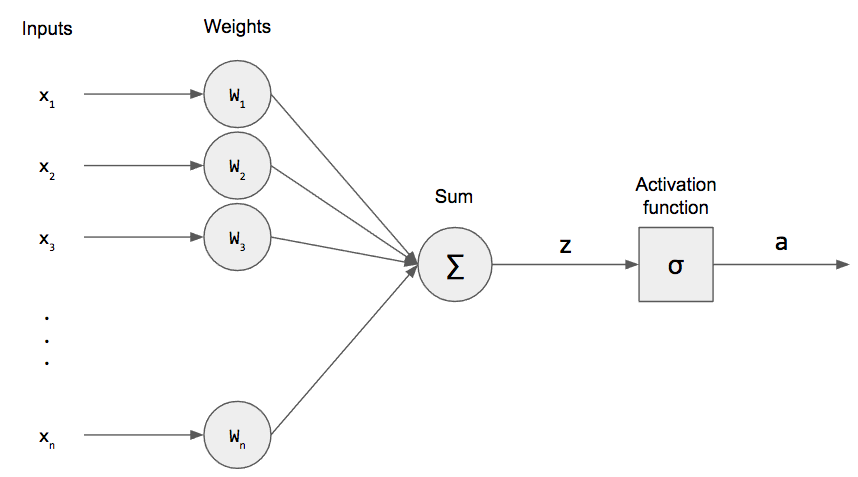
\includegraphics[width=\textwidth]{imgs/Single-Perceptron.png}
    \caption{Illustration of an LTU. The neurons are the building blocks of neural networks. 
    \\ Source: \url{https://gamedevacademy.org/perceptrons-the-first-neural-networks/}}
    \label{fig:perceptron}
\end{figure}

\par Now familiar with the mathematical expression of a perceptron, we slightly modify this latter to adapt it to the representation of a hidden layer of a neural network. Indeed, in the case of neural networks, the choice of the activation function is not limited to the step function. For the remainder of this chapter we therefore use the symbol $\sigma$ to denote any arbitrary activation function. We now consider a layer of $n$ LTUs followed by another one composed of $m$ LTUs. We write the output of the first layer in vector form:

\begin{equation}
\label{eq:output-vector}
\Vec{a}^{(1)} =
\begin{bmatrix}
o_1 \\
o_2 \\
\vdots \\
o_n
\end{bmatrix}
\end{equation}
If $\Vec{Z}^{(2)}$ is the output vector of the second layer before applying the activation function, where each entry of the vector $\Vec{Z}^{(2)}$ corresponds to an LTU, $\Vec{Z}^{(2)}$ can be expressed as follows:
\begin{equation}
\label{eq:ouput-layer}
 \Vec{Z}^{(2)} =
\begin{bmatrix}
z_1^{(2)} \\
z_2^{(2)} \\
\vdots \\
z_m^{(2)}
\end{bmatrix}
=
\begin{bmatrix}
o_1w_{11} + o_2w_{12} + \dots +o_i w_{1i} + b_1\\
o_1w_{21} + o_2w_{22} + \dots +o_i w_{2i} + b_2\\
\vdots \\
o_1w_{m1} + o_2w_{m2} + \dots +o_i w_{mi} + b_m
\end{bmatrix}
\end{equation}
where we have used Equation~\eqref{eq:post-synaptic-pot}. Indeed, for the $k^{\text{th}}$ LTU among the $m$ LTUs of the second layer, Equation~\eqref{eq:post-synaptic-pot} can be written as

\begin{equation*}
z_k = \sum_{i=1}^{m} x_i w_{ki} + b_k \text{ .}
\end{equation*}

The vector $\Vec{Z}^{(2)}$ can be rewritten as a dot product between the weight matrix $\mathbf{W}^{(2)}$ of layer 2 and the output vector $\Vec{a}^{(1)}$ given by Equation~\eqref{eq:output-vector}:

\begin{equation}
\label{eq:one-layer-output-detail}
\Vec{Z}^{(2)} =
\begin{bmatrix}
    w_{11} & w_{12} & \dots & w_{1n} \\
    w_{21} & w_{22} & \dots & w_{2n} \\
    \vdots & \vdots & \ddots & \vdots \\
    w_{m1} & w_{m2} & \dots & w_{jn}
\end{bmatrix}
\begin{bmatrix}
    o_1 \\
    o_2 \\
    \vdots \\
    o_n
\end{bmatrix}
+
\begin{bmatrix}
    b_1 \\
    b_2 \\
    \vdots \\
    b_m
\end{bmatrix}
\end{equation}
or equivalently

\begin{equation}
    \label{eq:output-layer-matrix}
    \Vec{Z}^{(2)} = \mathbf{W}^{(2)}\cdot \Vec{a}^{(1)} + \Vec{b}^{(2)}
\end{equation}

Finally, we can express the outputs of layer 2 in terms of the weights and biases of this layer and, the outputs of the previous one. For any layer $l$, and the preceding layer $l-1$, this can be written as:

\begin{equation}
\label{eq:output-any-layer}
\Vec{a}^{(l)} = \sigma^{(l)}\left(\Vec{Z}^{(l)}\right) = \sigma^{(l)}\left(\mathbf{W}^{(l)} \cdot \Vec{a}^{(l-1)} + \Vec{b}^{(l)}\right)
\end{equation}
where the activation function $\sigma$ is applied to each element of the vector $\Vec{Z_l}$.

A neural network is a mathematical function that can be represented as a graph of interconnected neurons (see Figure~\ref{fig:mlp}). Mathematically, this function can be described as a series of nested non-linear functions. The output of each function feeds into the input of the next function, and so on, until the final output of the network is produced. Formally, this is expressed as:

\begin{align}
f &\text{: } \mathbb{R}^n \to \mathbb{R}^m\nonumber\\
f &= g \circ f_L \circ f_{L-1} \dots f_2 \circ f_1 (x) \text{ with, }
\end{align}

\begin{align}
f_l &\text{: } \mathbb{R}^{n_l} \to \mathbb{R}^{n_{l-1}}\nonumber\\
f_l(x) &= \sigma^{(l)}(\mathbf{W}^{(l)} \cdot \Vec{x} + b^{(l)})
\end{align}

where $n$ is the dimension of the input $\Vec{x}$, $m$ is the dimension of the output $\Vec{y}$, $g$ is the \emph{output function}, and each $f_l$ is itself a composed multivariate function. In terms of what we have described with Equations~\eqref{eq:output-layer-matrix} and~\eqref{eq:output-any-layer}, this can be written in a more intuitive form as follows:

\begin{figure}[ht]
\centering
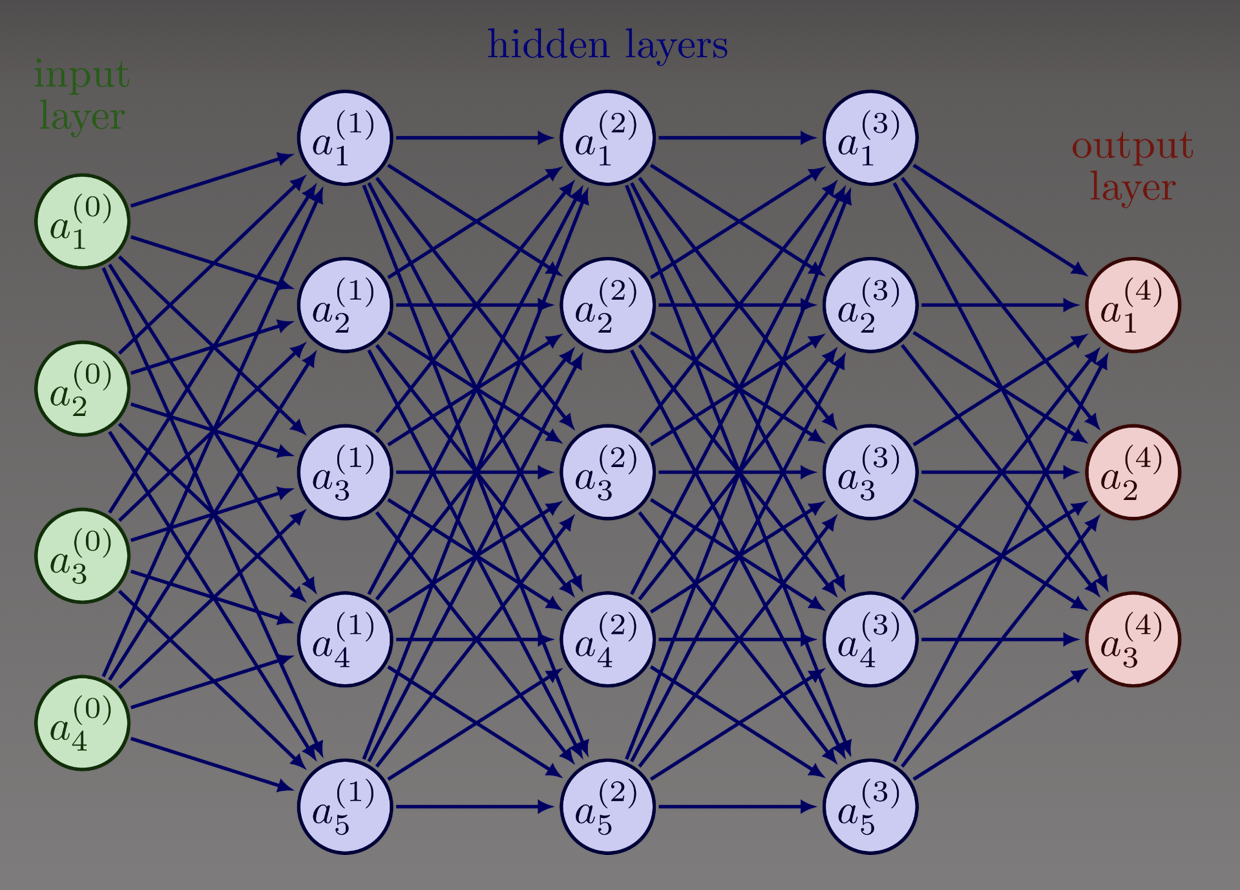
\includegraphics[width=\textwidth]{imgs/Architecture-perceptron-multi-couches-2.png}
\caption{Structure of a neural network with three hidden layers.}
\label{fig:mlp}
\end{figure}

\begin{equation}
\label{eq:mlp}
\hat{f}(\mathbf{x}) = g\left( \mathbf{W}^{(L-1)} \sigma^{(L-2)} \left( \cdots \sigma^{(2)} \left(
\mathbf{W}^{(2)} \sigma^{(1)} \left( \mathbf{W}^{(1)} \mathbf{x} + b^{(1)} \right) + b^{(2)} \right) \cdots \right) +
b^{(L-1)} \right)
\end{equation}
where $\hat{f}(\mathbf{x})$ denotes here the predicted output for a neural networks with $L$ layers. In other words, each hidden layer is calculated by applying a linear transformation $\mathbf{W}^{(l)} \cdot$ to the output of the previous layer, followed by a non-linear activation function $\sigma^{(l)}(\cdot)$. The final output is calculated by applying an output function $g$ to the output of the last hidden layer. The form of $g$ depends on the problem we aim to solve. In the case we are interested in, regression, $g$ is a simple linear function:

\begin{equation}
\label{eq:output-function}
g(\Vec{x}) = \mathbf{W}^{(L)} \cdot \Vec{x} + \Vec{b}^{(L)}
\end{equation}


We have formally described a forward pass of a Feed-forward Neural Network for input data $\Vec{x}$, given weights $w$ and biases $b$. These latter elements, which we will denote as $\theta$, can be initialized in various ways. We do not wish to delve into these details here and we just consider random initialization. Once initialized, we aim to adjust these weights and biases so that the function $\hat{f}(\Vec{x})$, approximated by the network, closely mirrors the true value of $f(\Vec{x})$. To this end, we require a method to tweak these parameters.

\subsection{Loss Function}

First, we quantify the error produced by the network using a \emph{loss function}, generally defined as follows:

\begin{equation}
\label{eq:def-loss-function}
\mathcal{L}(\theta) = \frac{1}{2n} \sum_{i=1}^n \left[\hat{y}_{\theta}^{(i)} - y^{(i)}\right]^2
\end{equation}
Here, $\theta$ represents the set of parameters, $\hat{y} = \hat{f}(\Vec{x})$ is the value predicted by the network, and $y=f(\Vec{x})$ is the actual value. We have employed the Mean Squared Error (MSE) as the loss function, commonly used for regression problems. The factor $1/2$ is added to simplify the factor of 2 that arises when calculating the gradient of $\mathcal{L}$.

\subsection{Gradient Descent}\label{subsec:gradient-descent}

We now have a function to measure the error made by the neural network. Naturally, for the network to be as efficient as possible, the error should be as low as possible. Therefore, we aim to minimize the loss function $\mathcal{L}$ from equation~\eqref{eq:def-loss-function}. The algorithm used for this process is called \emph{gradient descent}. This algorithm, proposed by Cauchy~\cite{cauchymethode} is based on the idea that if $F(\Vec{x})$ is a multivariate function defined and derivable in the vicinity of a point $\mathbf {a}$, then $ F(\mathbf {x} )$ decreases the fastest if we start from $\Vec{a}$ in the direction opposite to the gradient $\nabla F(\Vec{a})$.

In the parameter space $\theta$, we want to move towards a point $\Vec{\theta}$ that reduces the error $\mathcal{L}\left( \theta \right)$. Thus, following the gradient algorithm's principle, we want to change the point $\Vec{\theta}_{n}$'s coordinates in the direction given by $-\nabla \mathcal{L}(\Vec{\theta})$. We also need to define a unit length, or step size, by which we want to change the point's coordinates. This unit length is called the \emph{learning rate} and is often denoted as $\eta \in \mathbb{R}^+$. Finally, the change in parameters can be described as:

\begin{equation}
\label{eq:gradient-descent}
\Vec{\theta}_{n+1} = \Vec{\theta}_n - \eta \nabla \mathcal{L}(\Vec{\theta}_n)
\end{equation}

The choice of step size, $\eta$, is crucial. Using a small $\eta$ value could slow convergence and potentially trap the algorithm in a local minimum. On the other hand, choosing a large $\eta$ value could lead to divergence. The external parameters composing a neural network, and that are not trained, are called \emph{hyperparameters}. The choice of these hyperparameters is primordial and can decide whether a model is going to be successful or not.

\subsection{Gradient Descent Algorithms}
In practice, for networks containing a large number of parameters (on the order of $10^8-10^9$), iterating on each of these parameters following equation~\eqref{eq:gradient-descent} is not feasible. As a result, additional algorithms have been developed to circumvent this problem. We briefly present stochastic gradient descent, commonly used, as well as the Adam and L-BFGS algorithms, often employed in conjunction with PINNs.

\subsubsection{Stochastic Gradient Descent}
Stochastic Gradient Descent differs from ordinary gradient descent in that instead of taking into account all training examples to compute the gradient of the error, it selects just one example (or a small batch, in what's called the mini-batch method) at each iteration. Consequently, the gradient is computed and the weight updates are performed far more frequently, which can lead to faster convergence, though the individual steps are noisier. Mathematically, the iteration of a SGD step for a given weight is the same as for equation~\eqref{eq:gradient-descent}.

\subsubsection{Adaptive Moment Estimation}
The Adaptive Moment Estimation algorithm (Adam) is an optimization method introduced by Kingma and Ba~\cite{kingma2017adam}. This method is specifically designed for training deep neural networks. Its main advantage is that it adjusts the learning rate for each model weight individually, based on the estimates of the first moment (the mean) and the second moment (the uncentered variance) of the gradients.

The Adam algorithm can be detailed as follows:
\begin{enumerate}
    \item Initialize the first and second order moments as follows:
    \begin{itemize}
        \item $m_0=0$ (Initialize the 1st moment)
        \item $v_0=0$ (Initialize the 2nd moment)
    \end{itemize}
    \item For each iteration step $t$ (starting from $t=1$), compute the gradient $g_t$ of the error function with respect to the current parameters $\theta_t$.
    \item Update the moment estimates as follows:
    \begin{itemize}
        \item $m_t = \beta_1 \cdot m_{t-1} +(1-\beta_1) \cdot g_t$
        \item $v_t = \beta_2 \cdot v_{t-1} + (1-\beta_2) \cdot g_{t}^{2}$ 
        where $\beta_1$ and $\beta_2$ are hyperparameters controlling the decay of moments (typically 0.9 and 0.999 respectively).
    \end{itemize}
    \item Correct the moments for the initial bias towards zero as follows:
        \begin{itemize}
        \item $\hat{m}^t = \dfrac{m_t}{1 - \beta_{1}^{t}}$
        \item $\hat{v}^t = \dfrac{v_t}{1 - \beta_{2}^{t}}$
    \end{itemize}
    \item Lastly, update the parameters using the bias-corrected moments:

    $$\theta_{t+1} = \theta_t - \eta \cdot \dfrac{\hat{m}^t}{\sqrt{\hat{v}^t} + \epsilon}$$

where $\eta$ is the learning rate and $\epsilon$ is a small number to avoid division by zero (typically $10^{-8}$).
\end{enumerate}

The computation of first and second order moments enables Adam to adjust the learning rate of each parameter individually, which can help speed up the convergence of training, particularly in deep neural networks with many parameters.


\subsubsection{Limited-memory BFGS}
The BFGS (Broyden–Fletcher–Goldfarb–Shanno) algorithm is a quasi-Newtonian method that uses a formula to update the approximation of the  Hessian matrix (or its inverse) at each iteration. As an example, from an initial value $\Vec{x}_0$ and an approximated Hessian matrix $B_0$, the following iterations are repeated until $\Vec{x}$ converges towards the solution:
\begin{enumerate}
    \item Find the direction of descent $\Vec{p}_k$ by solving $B_k\Vec{p}_k = - \nabla f(\Vec{x}_k)$
    \item Perform a linear search to find the optimal step size $\alpha_k$, in the direction found in step 1, and then udpate
        $\Vec{x}_{k+1} = \Vec{x}_k + \alpha_k \Vec{p}_k = \Vec{x}_k + \Vec{s}_k$
    \item $\Vec{y}_k = f(\Vec{x}_{k+1}) - f(\Vec{x}_k)$
    \item $B_{k+1} = B_k + \left(\Vec{y}_k \Vec{y}_k^T\right)/\left(\Vec{y}_k^T \Vec{s}_k \right) - \left( B_k \Vec{s}_k\Vec{s}_k^TB_k\right)/\left(\Vec{s}_k^T B_k \Vec{s}_k\right)$
\end{enumerate} where $f(\Vec{x})$ is the function to minimize. This algorithm can also be expressed using the inverse Hessian matrix $H_k \equiv B_k^{-1}$. However, for problems with a large number of variables, storing and manipulating matrices $B_k$ or $H_k$ can be very costly in terms of memory and computation time.

This is where the L-BFGS (Limited-memory BFGS) algorithm~\cite{nocedal1980updating} comes into play. It is specifically designed for problems with a large number of variables. Instead of storing the complete inverse Hessian matrix, L-BFGS only stores a few vectors representing the differences in gradients and positions from previous iterations. Using these vectors, it's possible to compute an approximation of the inverse Hessian matrix, which allows for the next iteration to be performed.

The method used to compute this approximation is called the two-loop algorithm. The first loop, going from the current iteration to the current iteration minus $m$, uses the stored information to compute an approximation of the gradient. The second loop, going from the current iteration minus $m$ to the current iteration, uses the same information to compute the search direction.

\section{Back-propagation}\label{sec:backprop}

Backpropagation is an algorithm that enables the computation of the gradient of the error, thereby permitting the adjustment of network parameters according to~\eqref{eq:gradient-descent}. Prior to describing the algorithm, we compute the gradients with respect to each network parameter.

Starting from the gradient in Equation~\eqref{eq:gradient-descent} and employing the chain rule together with equation~\eqref{eq:post-synaptic-pot}, we may express:

\begin{equation}
\label{eq:gradient-wrt-weights}
\frac{\partial \L}{\partial w_{ik}^{(l)}} = \frac{\partial \L}{\partial z_{k}^{(l)}}\frac{\partial z_{k}^{(l)}}{\partial w_{ik}^{(l)}} = \frac{\partial \L}{\partial z_{k}^{(l)}} a_{k}^{(l-1)}
\end{equation}
Similarly, it can be shown that:

\begin{equation}
\label{eq:gradient-wrt-bias}
\frac{\partial \L}{\partial b_{k}^{(l)}} = \frac{\partial \L}{\partial z_{k}^{(l)}}\frac{\partial z_{k}^{(l)}}{\partial b_{k}^{(l)}} = \frac{\partial \L}{\partial z_{k}^{(l)}}
\end{equation}

Now, to fully express equations~\eqref{eq:gradient-wrt-weights} and~\eqref{eq:gradient-wrt-bias}, it suffices to determine $\frac{\partial \L}{\partial z_{k}^{(l)}}$. We aim to express this partial derivative in terms of data originating from the output layer. Information is propagated layer by layer, from right to left. Therefore, we need to express the derivative of the error with respect to $z^{(l)}$ based on this same quantity originating from layer $l+1$. This results in:

\begin{equation}
\label{eq:gradient-wrt-z}
\frac{\partial \L}{\partial z_{k}^{(l)}} = \sum_{m} \frac{\partial \L}{\partial z_{m}^{(l+1)}}\frac{\partial z_{m}^{(l+1)}}{\partial z_{k}^{(l)}} = \sum_{m} \frac{\partial \L}{\partial z_{m}^{(l+1)}}\frac{\partial z_{m}^{(l+1)}}{\partial a_{k}^{(l)}}\frac{\partial a_{k}^{(l)}}{\partial z_{k}^{(l)}}\text{ ,}
\end{equation}
where $m$ represents a neuron in layer $l+1$. Based on equation~\eqref{eq:output-any-layer} and equation~\eqref{eq:output-layer-matrix}, it follows that:

\begin{equation*}
\frac{\partial z_{m}^{(l+1)}}{\partial a_{k}^{(l)}} = w_{km}^{(l+1)}
\end{equation*}

and

\begin{equation*}
\frac{\partial a_{k}^{(l)}}{\partial z_{k}^{(l)}} = \sigma'(z_{k}^{(l)})
\end{equation*}

As a result, \eqref{eq:gradient-wrt-z} becomes:

\begin{figure}
    \centering
    \begin{tikzpicture}

        \node[draw,rectangle,minimum height=2cm,minimum width=3cm,align=center] (layer) at (0,0) {Layer $l$};
        
        \draw[<-] ([yshift=0.5cm]layer.west) -- ++(-2,0) node[midway,above] {$X^{(l)}=a^{(l-1)}$};
        \draw[->] ([yshift=-0.5cm]layer.west) -- ++(-2,0) node[midway,below] {$\frac{\partial E}{\partial X^{(l)}}$};
        
        \draw[->] ([yshift=0.5cm]layer.east) -- ++(2,0) node[midway,above] {$a^{(l)}$};
        \draw[<-] ([yshift=-0.5cm]layer.east) -- ++(2,0) node[midway,below] {$\frac{\partial E}{\partial a^{(l)}} $};
    \end{tikzpicture}
    \caption{Hidden layer $l$ of a neural network. Layer $l$ takes as input the data $\Vec{X}^{(l)}$, the output from the previous layer $l-1$, and outputs the vector $\Vec{a}^{(l)}$, as depicted by the upper arrows. The lower arrows illustrate the derivatives of the error with respect to the inputs of the previous layer, when backpropagation is performed.}
    \label{fig:illustration-layer-l}
\end{figure}

\begin{equation}
\label{eq:gradient-wrt-z-final}
\frac{\partial \L}{\partial z_{k}^{(l)}} = \sum_{m} \frac{\partial \L}{\partial z_{m}^{(l+1)}}w_{km}^{(l+1)}\sigma'(z_{k}^{(l)}) \text{ ,}
\end{equation}
where $\sigma'$ is the derivative of the activation function for hidden layers. It is assumed here that all hidden layers have the same activation function. If this is not the case, the expression remains the same, but one must indicate the function $\sigma$'s layer affiliation. The equations~\eqref{eq:gradient-wrt-weights},~\eqref{eq:gradient-wrt-bias} and~\eqref{eq:gradient-wrt-z-final} can be rewritten in a more concise manner using vector notation:

\begin{equation}
    \label{eq:gradient-wrt-weights-matrix}
    \frac{\partial \L}{\partial \Vec{W}^{(l)}} = \frac{\partial \L}{\partial \Vec{Z}^{(l)}} \cdot \Vec{a}^{(l-1)T}
\end{equation}

\begin{equation}
    \label{eq:gradient-wrt-bias-matrix}
    \frac{\partial \L}{\partial \Vec{b}^{(l)}} = \frac{\partial \L}{\partial \Vec{Z}^{(l)}}
\end{equation}

\begin{equation}
    \label{eq:gradient-wrt-z-final-matrix}
    \frac{\partial \L}{\partial \Vec{Z}^{(l)}} = \left(\Vec{W}^{(l+1)T} \cdot \frac{\partial \L}{\partial \Vec{Z}^{(l+1)}} \right) \odot \sigma'\left(\Vec{Z}^{(l)}\right)
\end{equation}
where $\odot$ is the Hadamard product. For the output layer, it simply comes:

\begin{equation}
\label{eq:gradient-output-layer}
    \frac{\partial\L}{\partial \Vec{W}^{(L)}} = \left(\hat{\Vec{y}} - \Vec{y}\right) g'(\Vec{a}^{(L)}) \Vec{a}^{(L-1)T}
\end{equation}

\subsubsection{Algorithm}
The backpropagation algorithm can be summarized in three main steps:
\begin{enumerate}
    \item Compute the forward pass for each input-output pair and store the results $\hat{y}$, $\Vec{a}^{(l)}$, $\Vec{Z}^{(l)}$ by proceeding from layer 1, the input layer, to layer $L$, the output layer.
    \item Compute the backpropagation phase for each input-output pair and store the results $\frac{\partial \L}{\partial w_{ik}^{(l)}}$ for each weight $ w_{ik}^{(l)}$ connecting node $i$ in layer $l-1$ to a node $k$ in layer $l$, by proceeding from layer $L$, the output layer, to layer 1, the input layer. This process is illustrated in Figure~\ref{fig:illustration-layer-l} for any given layer $l$. The steps for computing the backward phase are as follows: 
    \begin{enumerate}
        \item Evaluate the error term for the final layer using equation~\eqref{eq:gradient-output-layer}.
        \item Back-propagate the error terms for the hidden layers, starting from the last hidden layer $l=L-1$, by repeatedly applying equation~\eqref{eq:gradient-wrt-z-final}.
        \item Evaluate the partial derivatives of the error with respect to $w_{ik}^{(l)}$ using equation~\eqref{eq:gradient-wrt-weights}.
    \end{enumerate}
    \item Update the parameters according to equation~\eqref{eq:gradient-descent}.
\end{enumerate}

One full cycle of this algorithm is called an \emph{epoch}.
\section{Automatic Differentiation}\label{sec:AD}

Automatic-differentiation, also known as algorithmic differentiation (AD), is a collection of techniques used for evaluating the derivatives of a numerical function with high precision. It is grounded on the fact that every numerical function, regardless of its complexity, is ultimately a composition of several elementary functions (such as addition, multiplication, exponential, logarithm, etc.) and their derivatives are well known.

Automatic differentiation employs the chain rule to decompose the derivatives of complex functions into a series of derivatives of elementary functions. The idea is to apply the chain rule at each step of the function evaluation, storing intermediate results, which allows calculating the derivatives in a single pass through the function.

There are two modes of automatic differentiation. The \textbf{Forward mode} (or direct mode) computes the derivatives of all outputs with respect to one input. Suppose we have a function $\Vec{y} = f(\Vec{x})$, where $\Vec{x}$ is a vector and $\Vec{y}$ is a vector. The forward mode calculates the derivatives $\frac{\partial y_i}{\partial x_j}$ for all $i$ and a given $j$. On the other hand, the \textbf{Reverse mode} (or backward mode) computes the derivatives of one output with respect to all inputs. The reverse mode calculates the derivatives $\frac{\partial y_i}{\partial x_j}$ for a given $i$ and all $j$.

Both modes have their uses, but in deep learning, the reverse mode is most often used because we are typically interested in the gradient of a scalar cost function with respect to all model parameters.
Auto-differentiation has several advantages over other differentiation methods, including numerical and symbolic methods, which make it particularly appealing in deep learning.

\begin{itemize}
    \item Precision: Unlike numerical differentiation (which uses finite differences to estimate derivatives), AD is exact up to floating-point error. Numerical methods can introduce significant error, either due to machine precision (if the difference interval is too small), or due to a rough approximation of the derivative (if the interval is too large).
    \item Efficiency: AD is generally more efficient than symbolic differentiation, which can generate very complex expressions when working with complex functions or high dimensions (the so-called "expression swell" problem). AD, on the other hand, calculates the derivatives using a sequence of elementary operations (addition, multiplication, etc.) and corresponding derivation rules. This allows for more efficient calculation of derivatives and at a lower computational cost.
    \item Gradient calculation for multivariate functions: AD is particularly useful for calculating the gradient (or the Jacobian, or the Hessian) of multivariate functions. This is very relevant for deep learning, where we work with loss functions depending on thousands, or even millions of parameters.
\end{itemize}

Popular deep learning frameworks, such as PyTorch~\cite{NEURIPS2019_9015} that we use for this work, take advantage of automatic differentiation for fast computation. In fact, as mentioned in the introduction, one could argue that the use of PINNs, and their efficiency for quickly solving PDEs, relies strongly on this property of neural networks. 

\section{The Universal Approximation Theorem}\label{sec:univ-approx}
The universal approximation theorem asserts that a neural network with a single hidden layer can approximate any continuous function on compact subsets of $\mathbb{R}^n$, provided that the hidden layer's activation function is non-constant, bounded, and continuous.

The theorem is generally attributed to Cybenko~\cite{cybenko1989} for the case of sigmoid activation neural networks, and was extended by Hornik~\cite{hornik1991approximation} to cover the case of other activation functions.

To formalize it mathematically, let's suppose that $\phi : \mathbb{R} \rightarrow \mathbb{R}$ is a non-constant, bounded, and continuous activation function. For a continuous function $f : \mathbb{R}^n \rightarrow \mathbb{R}$ defined on a compact $K$ of $\mathbb{R}^n$, for any $\epsilon > 0$, there exists a natural number L and weight vectors $\Vec{w}^{(1)}, \dots, \Vec{w}^{(L)} \in \mathbb{R}^n$, scalars $b_1, \dots, b_L$ and $v \in \mathbb{R}$ such that:

\begin{equation}
| f(x) - F(x; v, w, b) | < \epsilon
\end{equation}
for every $x$ in $K$, where

\begin{equation}
F(x; v, w, b) = \sum_{k=1}^{L} v_k \phi(w_{k} x + b_k)
\end{equation}
Here, $F(x; v, w, b)$ represents the output of a one hidden layer neural network with $L$ neurons and an activation function $\phi$.

This means it's possible to construct a neural network that can approximate the function $f$ as closely as we desire, by appropriately choosing weights and biases. We assume this result to hold, as it motivates the use of neural networks for approximating potentials from Chapter~\ref{ch:galaxies-theory}, but the interested reader can find a formal proof in Appendix~\ref{app:approx-theorem}.
\chapter{Physics-Informed Neural Networks}\label{ch:pinns}

Although the idea of incorporating prior knowledge in a neural network for solving a PDE is not new~\cite{dissanayake1994}, we can consider the first Physics-Informed Neural Networks (PINNs) to have been introduced in 2017 in a two-part article~\cite{raissi_physics_2017,raissi_physics_2017-1}, which later merged into a single paper~\cite{raissi_physics-informed_2019}. PINNs are Neural Networks (NN) that encode the equations of physical models, including PDEs, as a component of the network itself. PINNs approximate the solutions of PDEs using a neural network, trained by minimizing a loss function. The specificity of PINNs lies in this loss function, which typically takes the form of a physical equation and also includes boundary conditions. This loss function is the key difference between PINNs and classical neural networks, which try to adjust their weights to best fit the data presented during training.
\par The PINN method is thus a meshless solution technique, finding the solutions to a PDE not by solving a governing equation, but by minimizing a certain loss function. This particular loss function restricts the space of acceptable solutions, thereby enabling the problem to be solved with satisfying accuracy.

\section{Definition}

One of the advantage of PINNs over typical neural networks is their ability to solve problems with very little, or noisy data. Due to their structure, PINNs are used to solve differential equations, which in their most general form can be written as~\cite{cuomo_scientific_2022}:

\begin{equation}
    \label{eq:pde-general}
    \begin{split}
        \mathcal{F}\left[ u(z); \lambda \right] &= f(z) \text{, } z \in \Omega\\
        \mathcal{B}\left[ u(z) \right] &= g(z) \text{, } z \in \partial\Omega
    \end{split}
\end{equation} where $u(z)$ denotes the solution to be determined, $\mathcal{F}[.;\lambda]$ is a non-linear operator parameterized by $\lambda$, $f$ is a function defining the problem data, $\mathcal{B}$ is an operator indicating a boundary, $g$ is a boundary function, and $\Omega$ is a subset of $\mathbb{R}^D$. Here, $z$ denotes the spatio-temporal domain. In our case, the equations are time-independent, and the integration will be carried out only over the spatial domain.

More concretely, the underlying methodology of PINNs can be summarized in three parts. First, the solution $u(z)$ is approximated by a neural network parameterized by a set of parameters $\theta$. Then, for a differential equation of the type
\begin{equation}
\label{eq:pde-exemple}
u_t + \mathcal{F}[u;\lambda] = 0\text{, } x\in \Omega\text{, } t \in [0, T]\text{,}
\end{equation} we set
\begin{equation}
p \coloneqq u_t - \mathcal{F}[u;\lambda] \text{.}
\end{equation} This function $p$ is referred to as a \emph{physics-informed neural network}. Finally, the network learns to approximate the differential equation by finding the set of parameters $\theta$ that minimizes the loss function $\mathcal{L}(\theta)$:

\begin{align}
    \label{eq:PINN-argmin-loss}
    \theta^* &= \underset{\theta}{\mathrm{argmin }} \text{ }\mathcal{L}(\theta) \nonumber \\
     &= \underset{\theta}{\mathrm{argmin }} \left( \omega_{\mathcal{F}}\mathcal{L}_{\mathcal{F}}(\theta) + \omega_{\mathcal{B}}\mathcal{L}_{\mathcal{B}}(\theta) + \omega_{data}\mathcal{L}_{data}(\theta) \right)\text{ ,}
\end{align}
where the $\omega_i \text{, } i \in \{\mathcal{F}, \mathcal{B}, \mathrm{data}\}$  are weights for the specific losses $\L_i$, respectively defined for the PDE residual, the boundary and the data. Their expressions are detailed in the following section.

\section{Properties}

\subsubsection{Loss Function}
We note that unlike a typical loss function, we have for the PINNs a weighted sum of several loss functions, each corresponding to one of the training contributions mentioned above; the governing equation residual, the boundary conditions, and the data points.

We first focus on the loss function arising from the difference between the network's prediction and the governing differential equation $\mathcal{F}$ :
\begin{equation}
    \label{eq:pde-loss}
    \mathcal{L}_{\mathcal{F}}(\theta) = MSE_{\mathcal{F}} = \dfrac{1}{N_c}\sum^{N_c}_{i=1} \left\|\mathcal{F}(\hat{u}_{\theta}(z_i)) - f(z_i)\right\|^2
\end{equation} where $N_c$ is the number of points where the PDE residual is evaluated in the domain. These points are called \emph{collocation points}. MSE is the commonly used mean square error. This loss function is computed by taking advantage of the auto-differentiation properties of neural networks (see Section~\ref{sec:AD}) to compute the partial derivatives of $\hat{u}_{\theta}(z)$. Similarly, we then have the error coming from the boundary conditions:

\begin{equation}
    \label{eq:boundary-loss}
    \mathcal{L}_{\mathcal{B}}(\theta) = MSE_{\mathcal{B}} = \dfrac{1}{N_B}\sum^{N_B}_{i=1} \left\|\mathcal{B}(\hat{u}_{\theta}(z_i)) - g(z_i)\right\|^2
\end{equation} where $N_B$ is naturally the number of points used to represent the boundary conditions. Finally, the error due to discrepancies with the data points takes the following form:

\begin{equation}
    \label{eq:data-loss}
    \mathcal{L}_{data}(\theta) = MSE_{data} = \dfrac{1}{N_d}\sum^{N_d}_{i=1} \left\|\hat{u}_{\theta}(z_i)) - u^{*}_i\right\|^2
\end{equation} where $N_d$ is the number of data points. Depending on the problem setup, one can choose higher or lower values for the weights $\omega_i \text{, } i \in \{\mathcal{F}, \mathcal{B}, \mathrm{data}\}$, always with $|\omega_i| \leq 1$. For example, one can decrease the value of $\omega_{\mathcal{F}}$ if the model's PDE is deemed unreliable to describe the system. Or decrease $\omega_{data}$ if the data are noisy. In an inverse problem, PINNs can be used to model the data, while simultaneously solving the PDE. In other words, in an inverse problem a PINN can determine the parameters $\lambda$ from Equation~\eqref{eq:pde-exemple} given some simulation data. Lastly, it is worth noting that in the case of a forward problem, the error related to the data can also represent the boundary conditions. In our case, we will indeed rather use the error $\mathcal{L}_{data}(\theta)$ estimated at the borders, than a loss function as given by equation~\eqref{eq:boundary-loss}. We will then write our loss function as follows:

\begin{equation}
    \label{eq:loss-galaxy}
    \mathcal{L}(\theta) = \dfrac{1}{N_c}\sum^{N_c}_{i=1} \left\|\nabla^2 \hat{\Phi}(z_i) - 4 \pi G \rho(z_i) \right\|^2 + \dfrac{1}{N_B}\sum^{N_B}_{i=1} \left\|\hat{\Phi}(z_i) - \Phi_i \right\|^2
\end{equation}
where $\hat{\Phi}(z_i)$ is the predicted gravitational potential at point $z_i$, and $\Phi_i$ is the real value of the potential at that same point. The procedure described above is summarized in Figure~\ref{fig:loss-pinn}.

\begin{figure}[ht]
    \centering
    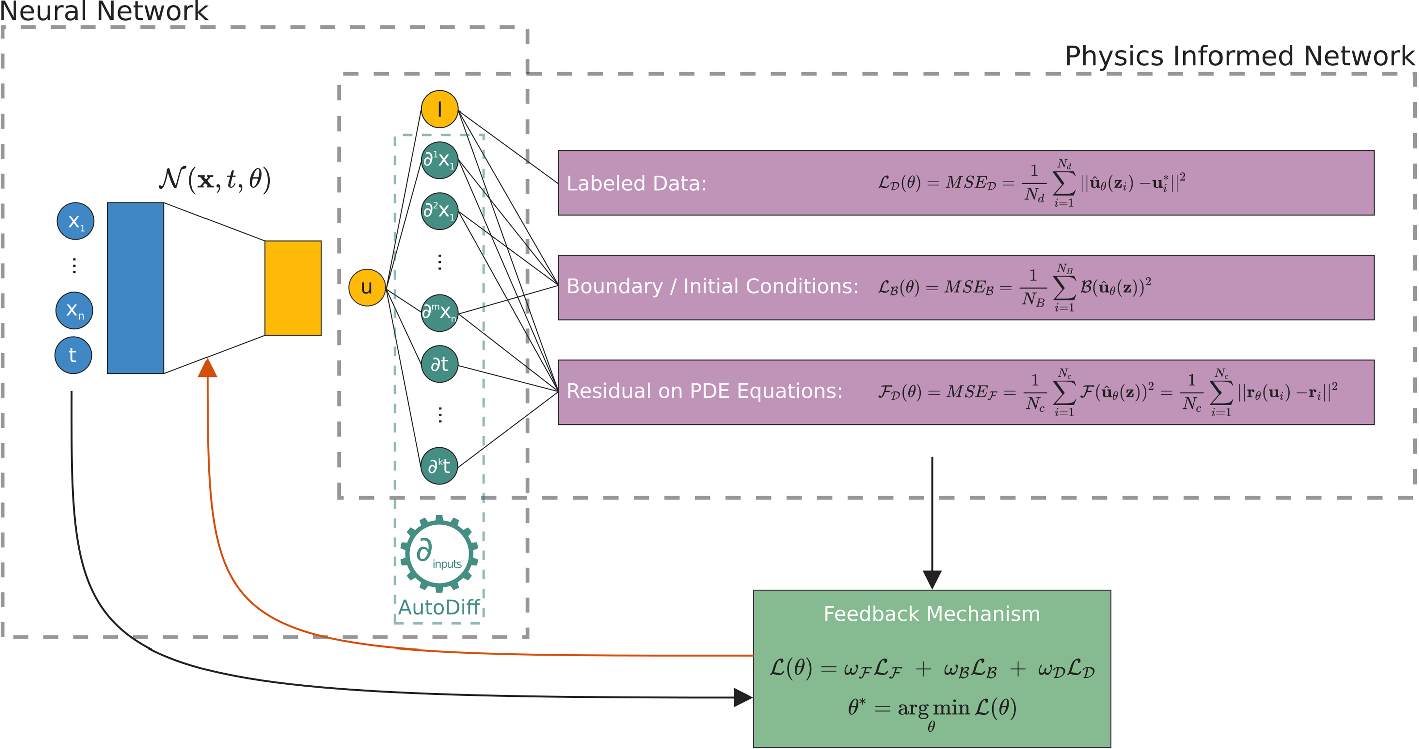
\includegraphics[scale=0.25]{imgs/training-pinn-schema.png}
    \caption{Structure and training procedure of a PINN. The fundamental difference with a typical neural network is the inclusion of a differential equation and boundary terms in the loss function. \textit{Illustration from~\cite{cuomo_scientific_2022}}.}
    \label{fig:loss-pinn}
\end{figure}

\subsubsection{Optimization}

As previously indicated, solving a PDE with a PINN comes down to minimizing the loss function $\mathcal{L}(\theta)$; it's therefore an optimization problem. This process is called \emph{training}. As described in Chapter~\ref{ch:neural-networks}, there are several algorithms to find the minimum of the loss function. However, in most cases~\cite{cuomo_scientific_2022} PINNs are trained using the Adam algorithm, or the Limited-memory Broyden-Fletcher-Goldfarb-Shanno (L-BFGS) method. The Adam approach combines an adaptive learning rate with momentum methods, while the L-BFGS method is a quasi-Newtonian optimization algorithm~\cite{cuomo_scientific_2022}. These two algorithms are predominantly used due to their speed of convergence, compared to a simple gradient descent. Particularly, it is shown in~\cite{he_physics-informed_2020} that in the case where the number of residuals or data points is limited, the L-BFGS-B algorithm\footnote{The L-BFGS-B algorithm extends the L-BFGS algorithm to handle simple box constraints.} is more efficient, with a faster convergence rate and reduced computational cost.

\subsubsection{Activation Function}

As mentioned in chapter~\ref{ch:neural-networks}, there are many possible activation functions to build a model with a neural network. In our case we want our activation function to be at least of class $\mathcal{C}^2$, twice differentiable, since we take the gradient of $\hat{\Phi}(z)$ twice when calculating the Laplacian. Thus, we will mainly use the hyperbolic tangent function in our work, and study the effect of sigmoid, silu or even log-sigmoid functions on the accuracy of our model.

%\subsubsection{Error (optional)}

%We will not detail in this work a formal analysis on the error of PINNs and their limitations. However, this component of the study of PINNs is where the most work remains to be done. Therefore, we wish to provide some theoretical results to support the consistency of our study, but the interested reader can find an exhaustive description of the actual work in this field in~\cite{cuomo_scientific_2022}. In particular, a recent result from~\cite{de_ryck_approximation_2021} proves that the difference $\hat{u} - u$ tends to $0$ when the width of the neural network, with a hyperbolic tangent activation function, tends to infinity. Thus, we ensure that by choosing a neural network, with two hidden layers and a tanh activation function, with a sufficient number of neurons, we will be able to approximate the gravitational potential as closely as desired.

\subsubsection{Architecture}

Since their first implementation in 2017~\cite{raissi_physics_2017} with a Feed-Forward Neural Network (FFNN), PINNs have evolved and transformed. Although the majority of PINNs still use an FFNN architecture, there exist now numerous other implementations with different architectures; convolutional networks, recurrent networks, Bayesian networks, etc. Interested readers can find an exhaustive list of these architectures in the review article~\cite{cuomo_scientific_2022}. For our part, we will use an FFNN, in which each neuron is connected to all the neurons in the next layer, as described in chapter~\ref{ch:neural-networks}. Although the idea of this work is not to strive to find the hyperparameters that provide the optimal results, we will look at the impact that some of these parameters, such as the activation function or the width of the network, have on the accuracy of the PINN.

\section{Applications}\label{ch:applications}


\subsection{Hernquist Model}\label{sec:hernquist}

\begin{frame}{Hernquist Model}
        The differential equation  we aim to solve:

    \begin{equation*}
        \dfrac{\dd}{\dd s}\left(s^2 \dfrac{\dd \Phi'}{\dd s}\right) = \dfrac{2s}{(s+1)^3}
    \end{equation*} which yields the following loss function for the PINN:
    \begin{equation*}
            \mathcal{L}(\theta) = \dfrac{1}{N_c}\sum^{N_c}_{i=1} \left|\dfrac{\dd}{\dd s_i}\left(s_{i}^{2} \dfrac{\dd \hat{\Phi}'}{\dd s_i}\right) - \dfrac{2s_i}{(s_i+1)^3} \right|^2 + \dfrac{1}{N_d}\sum^{N_d}_{i=1} \left|\hat{\Phi}'(s_i) - \Phi'_i \right|^2
    \end{equation*}
\end{frame}

\begin{frame}{Hernquist - Training}
\begin{columns}
    \column{\moit}
    \begin{figure}
        \centering
        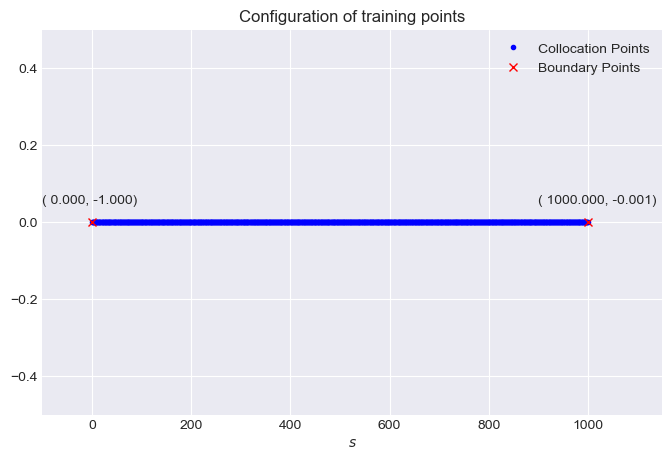
\includegraphics[width=\textwidth]{imgs/training-points-hernquist.png}
        \caption{Configuration of training points in the spatial domain $s \in [0, 1000]$.}
        \label{fig:training-points-hernquist}
    \end{figure}
    \column{\moit}
    \begin{figure}
        \centering
        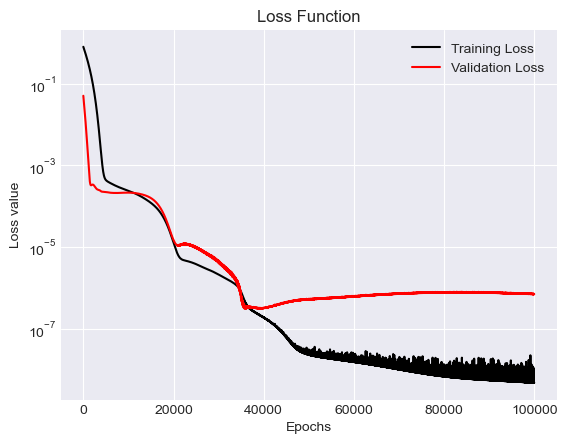
\includegraphics[width=\textwidth]{imgs/error-hernquist.png}
        \caption{Evolution of training and validation error functions.}
        \label{fig:losses-hernquist}
    \end{figure}
\end{columns}
\end{frame}

\begin{frame}{Hernquist - Results}

\begin{figure}
    \centering
        \begin{subfigure}[b]{0.49\textwidth}
        \centering
        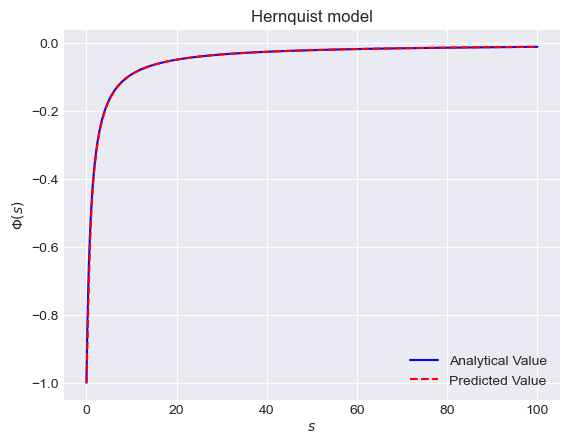
\includegraphics[width=\textwidth]{imgs/test-plot-hernquist.png}
        \caption{Comparison between the actual value of the potential and that predicted by the PINN on a test domain $s \in [0, 100]$.}
        \label{fig:test-plot-hernquist}
        \end{subfigure}
    \hfill
    \begin{subfigure}[b]{0.49\textwidth}
        \centering
        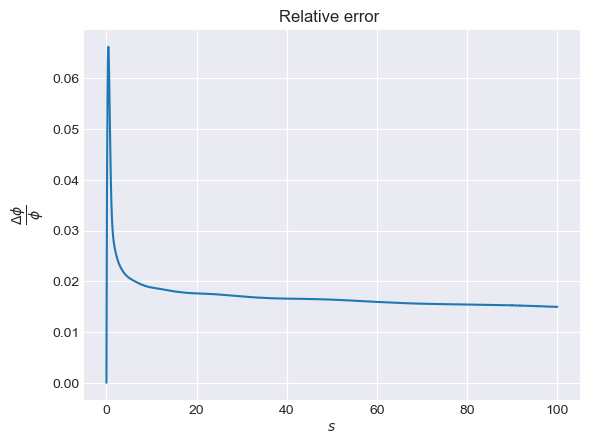
\includegraphics[width=\textwidth]{imgs/relative-error-hernquist.png}
        \caption{Relative error along the domain $s$. The average error over the entire domain is $1.71$\%.}
        \label{fig:relative-error-hernquist}
    \end{subfigure}
    \caption{As illustrated by the two figures presented, a PINN is capable of predicting with acceptable accuracy the value of the Hernquist potential $\Phi$ at a given point in a domain in which it has been trained.}
    \label{fig:three graphs}
\end{figure}
\end{frame}


\begin{frame}{Dehnen Model}
\only<1>{The differential equation we want to solve:

\begin{equation*}
    \dfrac{\dd}{\dd s}\left(s^2 \dfrac{\dd \Phi'}{\dd s}\right) = \dfrac{2s^{2-\gamma}}{(1+s)^{4-\gamma}}
\end{equation*}}

The exponent $\gamma$ drastically changes the dynamics of the potential:
\only<2>{
\begin{figure}
\centering
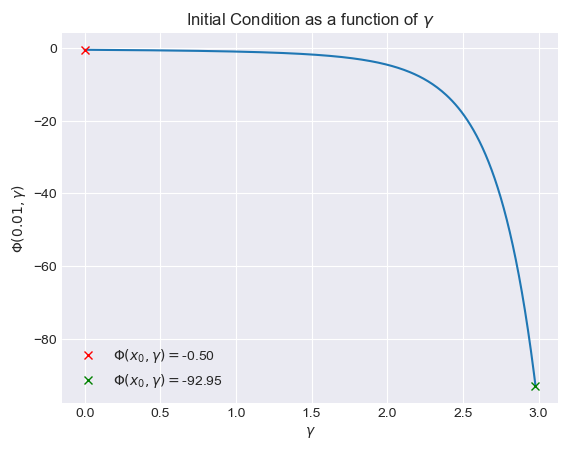
\includegraphics[width=0.6\textwidth]{imgs/gamma-vs-x0-dehnen.png}
\caption{Value of the gravitational potential at $s_0 = 0.01$ for different values of $\gamma \in [0, 3[$. Predicting the potential value at $s_0=0$ is a complex task for the PINN given the high sensitivity of $\Phi(s_0, \gamma)$ to the value of $\gamma$.}
\label{fig:gamma-vs-x0-dehnen}
\end{figure}}
\end{frame}
\subsection{Dehnen Model}\label{sec:dehnen}


\begin{frame}{Dehnen - Training}
    \begin{columns}
        \column{\moit} \begin{figure}
            \centering
            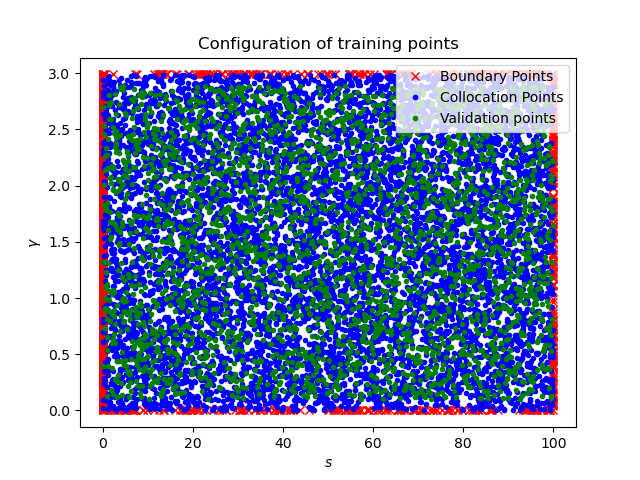
\includegraphics[width=\textwidth]{imgs/training-points-dehnen.png}
            \caption{Distribution of training and validation points on the domain.}
            \label{fig:training-points-dehnen}
        \end{figure}
        \column{\moit} \begin{itemize}
            \item Problems to obtain satisfactory results
            \item No observable improvement by manually tuning hyperparameters
            \item Change the penality of loss function to MAE
        \end{itemize}
    \end{columns}
\end{frame}



\begin{frame}{Dehnen - Results}
    \begin{columns}
    \column{\moit}
        \begin{figure}
            \centering
            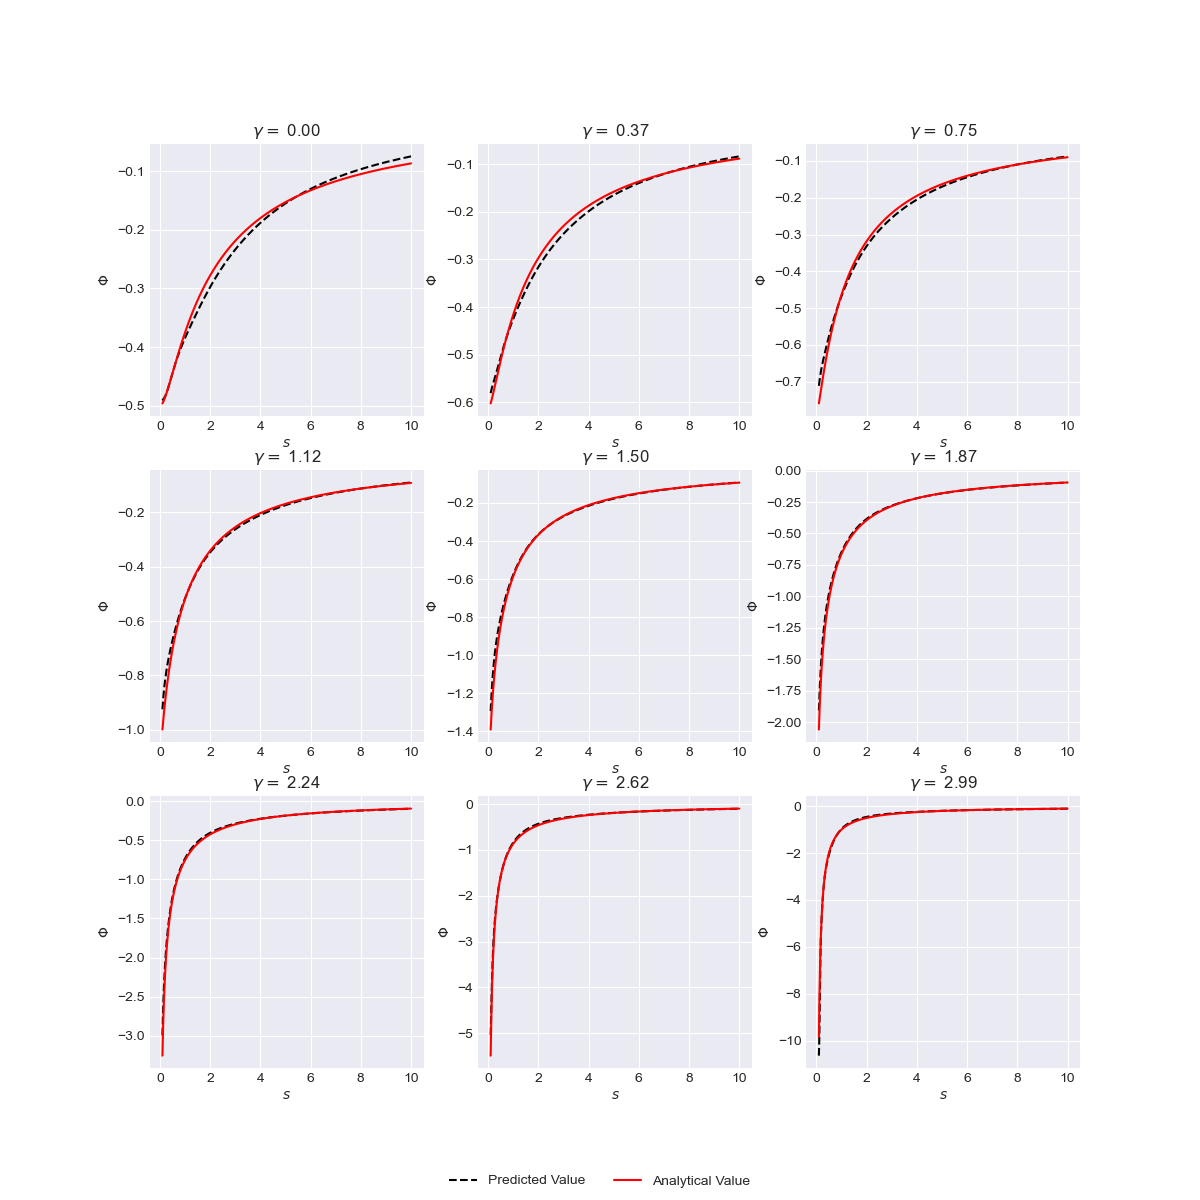
\includegraphics[width=\textwidth]{imgs/test-plot-dehnen.png}
            \caption{Comparison between the real value of the potential and that predicted by the PINN on a test domain $s \in [0, 10]$ for different values of $\gamma$.}
            \label{fig:test-plot-dehnen}
        \end{figure}
    \column{\moit} 
        \begin{figure}
            \centering
            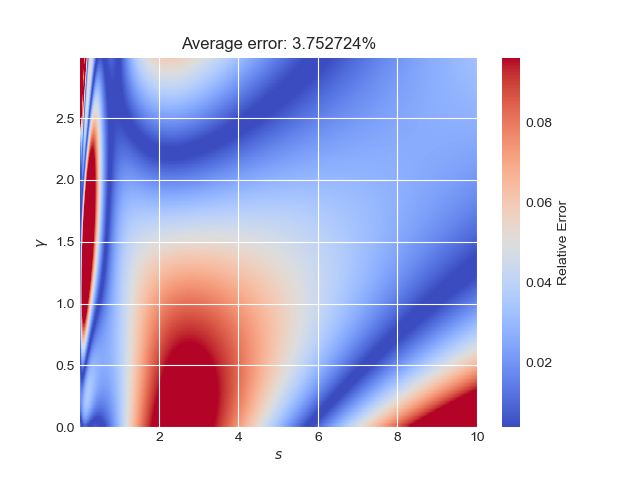
\includegraphics[width=\textwidth]{imgs/relative-error-dehnen.png}
            \caption{Relative error on the $s \times \gamma$ grid. The relative error can reach nearly 20\%.}
            \label{fig:relative-error-dehnen}
        \end{figure}
    \end{columns}
\end{frame}



\subsection{Thick Exponential Disk}\label{sec:disk}

\begin{frame}{Thick Exponential Disk Model}
    We aim to solve the following differential equation:
    \begin{equation*}
        \dfrac{1}{R'} \dfrac{\partial}{\partial R'} \left(R' \dfrac{\partial \Phi'}{\partial R'}\right) + \dfrac{1}{\eta^{2}}\dfrac{\partial^2 \Phi'}{\partial z'^2} = e^{-R'} \cosh^{-2}{z'}
\end{equation*} 
$z' = z/z_d$, $R' = R/R_d$, $\eta = z_d/R_d $ and $\phi'= \frac{\phi}{G M_d/z_d}$
\end{frame}

\begin{frame}{Thick Exponential Disk - Training}
    \begin{columns}
        \column{0.4\textwidth} 
        \begin{itemize}
            \item Wish to obtain the best solution possible
            \item Need to find the best set of hyperparameters
            \item Wish to understand the impact of certain hyperpameters on the error

        \end{itemize}
        \column{0.6\textwidth}
        Simple grid search for hyperparameters fine-tuning
        \begin{table}[h]
        \centering
        \scalebox{0.8}{
        \begin{tabular}{|l|c|}
        \hline
        \textbf{Parameters} & \textbf{Values} \\
            \hline
            \# Neurons & 32, 64, 128 \\
            \hline
            \# Layers & 1, 2, 3, 4, 5, 6 \\
            \hline
            Learning Rate & 1e-4, 1e-5, 1e-6 \\
            \hline
            Loss Func. & mse \\
            \hline
            Activation & Tanh, Sigmoid, SiLU, LogSigmoid \\
            \hline
        \end{tabular}}
        \label{tab:fine-tuning}
        \end{table}
    \end{columns}
\end{frame}

\begin{frame}{Thick Exponential Disk - Results}
    \only<1>{
    Two kind of solutions:
    \begin{enumerate}
        \item Computing an approximate solution efficiently $\rightarrow 3 \times 32$ NN, ~ 80 seconds of computation and average error of $1.85\%$.
        \item Find a model giving the smallest error possible $\rightarrow$ fine-tuning, $6 \times 128$ NN, ~ 20 minutes of training and average error of $0.36\%$.
    \end{enumerate}}
    \only<2>{
    \begin{figure}
        \centering
        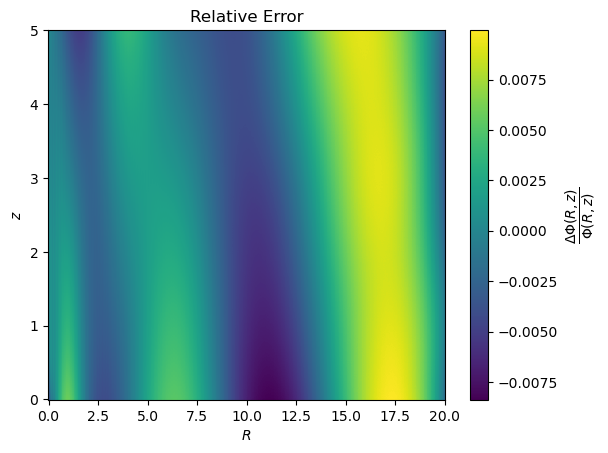
\includegraphics[width=0.6\textwidth]{imgs/relative-error-expdisc.png}
        %\caption{Relative error on the $R' \times z'$ grid. The average error over the entire domain is 0.36\%, and the maximum error is 0.99\%.}
        \label{fig:relative-error-expdisc}
    \end{figure}
    Satisfactory result, but parameter $\eta$ is here fixed $\rightarrow$ Need to extend the PINN !
    }
    
\end{frame}

\begin{frame}{Hyperparameters}
    How do hyper-parameters influence the relative error? 
    \only<1>{The activation function:
    \begin{figure}
        \centering
        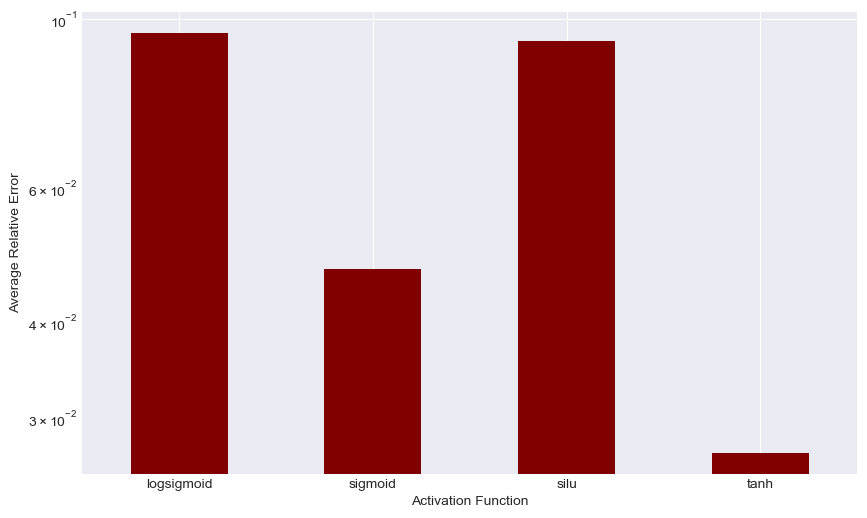
\includegraphics[scale=0.5]{imgs/function-error-expdisc.png}
        %\caption{Average relative error for certain activation functions.}
        \label{fig:function-error-expdisc}
    \end{figure}
}
    \only<2>{The learning rate:
    \begin{figure}
        \centering
        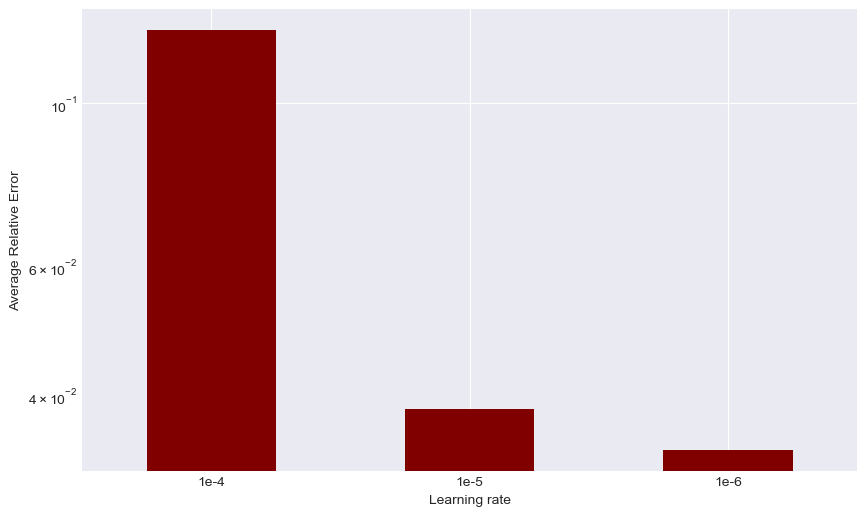
\includegraphics[scale=0.5]{imgs/learning-rate-expdisc.png}
        %\caption{Average relative error for different learning rates.}
        \label{fig:learning-rate-expdisc}
    \end{figure}
    }

    \only<3>{The number of neurons per layer:
     \begin{figure}
        \centering
        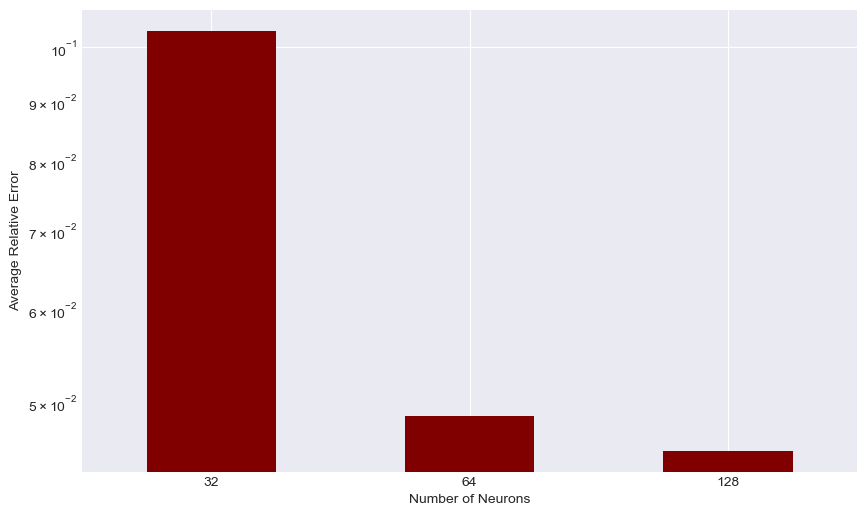
\includegraphics[scale=0.4]{imgs/neurons-error-expdisc.png}
        %\caption{Influence of the number of neurons per hidden layer on the average relative error.}
        %\label{fig:neurons-error-expdisc}
    \end{figure}
    }
    \only<4>{The number of hidden layers:
    \begin{figure}
        \centering
        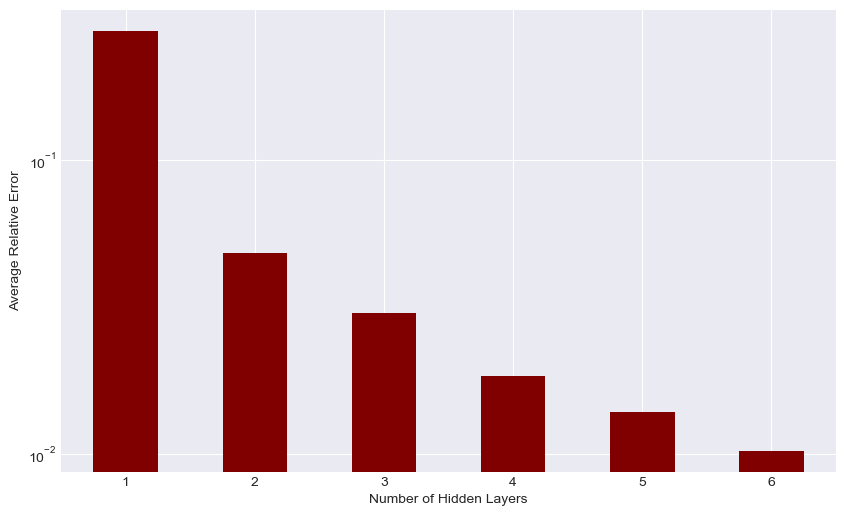
\includegraphics[scale=0.4]{imgs/layers-error-expdisc.png}
        %\caption{Influence of the number of hidden layers on the average relative error.}
        %\label{fig:layers-error-expdisc}
        \end{figure}
    }
    \only<5>{Is it solely the total number of neurons, or does the architecture have an impact?
    \begin{figure}
        \centering
        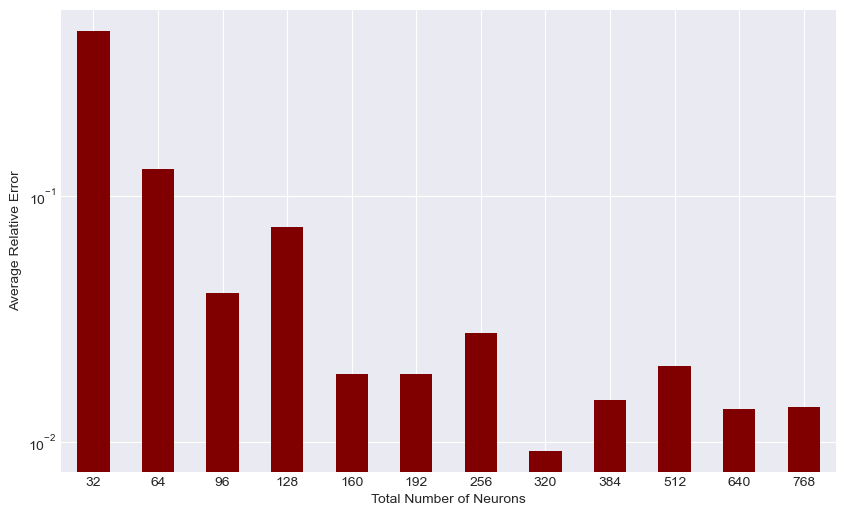
\includegraphics[width=0.65\textwidth]{imgs/tot-neurons-error.png}
        %\caption{Evolution of the average relative error as a function of the total number of neurons in the PINNs.}
        \label{fig:tot-neurons-error}
    \end{figure}
    }
\end{frame}


\chapter{Conclusion}\label{ch:conclusion}

In this trailblazing study, we have taken the initial stride towards the development of novel tools for simulating galaxies. The proficiency of Physics-Informed Neural Networks (PINNs) in solving the gravitational Poisson equation~\eqref{eq:poisson_eq_general} has been substantiated for three distinct density profiles, two of which are spherically symmetric and one that is axisymmetric. The initial two models yield comparatively accurate results - averaging 1.71\% and 3.75\% respectively - without necessitating any fine-tuning. Further research could potentially diminish the error of these PINNs, however, given that these two models admit an analytical solution, we did not undertake to optimize them in this particular study. The Poisson equation that describes the exponential thick disc model, on the other hand, does not admit an analytical solution, and hence the associated PINN can serve a genuine practical utility.

To confirm that the error could be considerably reduced, we conducted a rudimentary grid search, according to the parameters displayed in Table~\ref{tab:fine-tuning}. This grid search allowed us to select a PINN model that delivers an average relative error of 0.36\%, with a maximum of merely 0.99\%. These results are obtained for a fixed value of $\eta$ (see equation~\eqref{eq:poisson-exp-disc-final}), a ratio of the model's scale lengths. Despite the success of the two-parameter PINN, it remains to be demonstrated that the extension of this PINN to three dimensions performs as satisfactorily. This extension is an excellent opportunity to underscore once again the adaptability of PINNs. Utilizing techniques such as the finite difference method, it is not straightforward to modify the code to include an additional dimension. With a PINN, however, one merely needs to adjust the input data or possibly the PDE residual.


\section{Outlooks and Future Works}

As previously mentioned, this work is innovative in many respects, and while we have taken the initial step by demonstrating the capability of PINNs to solve certain gravitational potentials, there is still much to be accomplished. In the domain of galaxy modeling, one could first extend the work performed to other non-analytical models, or attempt to solve the Jeans equations, which are used to describe the velocity field of a galaxy. More generally, within the field of PINNs, there are several uncharted paths to investigate. We discuss a few of these in this section.
\subsection{Hyperparameters}
While the Hernquist~\cite{hernquist_analytical_1990} and Dehnen~\cite{dehnen_family_1993} profiles admit analytical solutions, it would nonetheless be necessary to undertake an extensive fine-tuning of the hyperparameters to ascertain whether the PINN can achieve an arbitrarily high precision or whether it is bounded. Additionally, the search for hyperparameters for the exponential thick disc allowed us to study the influence of these parameters on the PINN error (see Figures~\ref{fig:hyperparametres-vs-error} and~\ref{fig:tot-neurons-error}). This empirical exploration enables us to note that in the case of the exponential thick disc, the tanh function generally performs significantly better than the sigmoid or SiLU functions. We also observe that the network width-the number of neurons per layer-seems to cease improving the precision beyond a certain threshold. It appears that for an equivalent number of neurons, it is preferable to increase the network depth, as illustrated in Figure~\ref{fig:tot-neurons-error}. Ultimately, although literature~\cite{he_physics-informed_2020} suggests that the L-BFGS-B optimizer is the most effective under conditions similar to ours, it was unable to solve the Poisson equation for the Hernquist model. 
\par More broadly, a dedicated and rigorous exploration of hyperparameters would be beneficial and could potentially contribute to a deeper understanding of the operational intricacies of PINNs.

\subsection{Theory and Interpretability}
The empirical findings discussed above illustrate the challenges encountered with PINNs. Indeed, there are very few theoretical results that provide bounds on the error made by the PINN. A notable result is that of~\cite{de_ryck_approximation_2021}, which provides a bound on the PINN error as a function of the total number of neurons in the network. In another more recent paper~\cite{de_ryck_error_2023}, the same authors demonstrate that there exists a neural network approximating the classical solution of the Navier-Stokes equation such that the generalization error and the training error of the PINN are arbitrarily small. Explicit bounds on the number of neurons and network weights are also provided, depending on the error tolerance and the Sobolev norms of the underlying Navier-Stokes equation. However, these results are limited to two-layer networks using the tanh activation function and therefore do not elaborate on the influence of network width or depth in relation to the total number of neurons in the network. Ultimately, new theoretical results would be beneficial and necessary to prevent PINNs from remaining somewhat of a black box that cannot be fully deciphered.

\subsection{Inverse Problem}

While in this study we have demonstrated the proficiency of PINNs as solvers for swiftly simulating intricate systems, thereby allowing them to be used for parameter estimation, we have not yet fully harnessed the power of PINNs. Indeed, as outlined in Chapter~\ref{ch:pinns}, when furnished with simulation data of a system, a PINN possesses the capability to discern the parameters of a PDE. This is the so-called Inverse Problem. Therefore, if the end goal is to utilize the solution from a PINN over a given domain for parameter estimation, it naturally prompts the question as to whether it is feasible to utilize the inverse problem for ascertaining the parameters of a potential-density pair.

\appendix 
\chapter{Solving the Poisson equation}\label{app:poisson}
\chapter{The Universal Approximation Theorem}\label{app:approx-theorem}
\chapter{Latin Hypercube Sampling}\label{app:lhs}

\newpage
\Large
\noindent
\textbf{Declaration of authorship} 
\vspace{0.5cm}
\noindent
\normalsize

I hereby declare that the report submitted is my own unaided work. All direct 
or indirect sources used are acknowledged as references. I am aware that the 
Thesis in digital form can be examined for the use of unauthorized aid and in 
order to determine whether the report as a whole or parts incorporated in it may 
be deemed as plagiarism. For the comparison of my work with existing sources I 
agree that it shall be entered in a database where it shall also remain after 
examination, to enable comparison with future Theses submitted. Further rights 
of reproduction and usage, however, are not granted here. This paper was not 
previously presented to another examination board and has not been published.

\bibliographystyle{apalike}
\bibliography{references}
%\printglossary[type=\acronymtype]
\end{document}
